\documentclass[a4paper]{article}
\usepackage{geometry}
\geometry{
	a4paper,
	total={170mm,257mm},
	left=27mm,
	right=30mm,
	top=30mm,
	bottom= 30mm
}
\usepackage{lipsum}
\usepackage{tabu}
\usepackage[english]{babel}
\usepackage[utf8]{inputenc}
\usepackage[parfill]{parskip}
\usepackage{longtable}
\usepackage{amsmath}
\usepackage{graphicx}
\usepackage{enumitem}
\usepackage[colorinlistoftodos]{todonotes}
\usepackage{tikz}
\newcommand*\circled[1]{\tikz[baseline=(char.base)]{
		\node[shape=circle,draw,inner sep=0.5pt] (char) {#1};}}
\usetikzlibrary{fit,positioning}
\usepackage{authblk}
\usepackage{natbib}
\usepackage[algo2e]{algorithm2e}
\usepackage{algorithmic}  
\usepackage{algorithm}
\usepackage{comment}
\usepackage{bbm}
\usepackage{array}% http://ctan.org/pkg/array
\makeatletter
\g@addto@macro{\endtabular}{\rowfont{}}% Clear row font
\makeatother
\newcommand{\rowfonttype}{}% Current row font
\newcommand{\rowfont}[1]{% Set current row font
	\gdef\rowfonttype{#1}#1%
}
\newcolumntype{L}{>{\rowfonttype}l}
\title{A Network Model for Dynamic Textual Communications \\with Application to
	Government Email Corpora\footnote{\noindent Prepared for presentation at the New Directions in Analyzing Text as Data (Text As Data 2017). This work was supported in part by the University of Massachusetts Amherst Center for Intelligent Information Retrieval and in part by National Science Foundation grants DGE-1144860, SES-1619644, and CISE-1320219. Any opinions, findings, and conclusions or recommendations are those of the authors and do not necessarily reflect those of the sponsors. }}

\author[1]{Bomin Kim}
\author[3]{Aaron Schein}
\author[1]{Bruce Desmarais}
\author[2,3]{Hanna Wallach}
\affil[1]{Pennsylvania State University}
\affil[2]{Microsoft Research NYC}
\affil[3]{University of Massachusetts Amherst}

\begin{document}
\setlength{\parindent}{0pt}
\maketitle
\begin{abstract}
	
	\noindent In this paper, we introduce the interaction-partitioned topic model
	(IPTM)---a probabilistic model for who communicates with whom about
	what, and when. Broadly speaking, the IPTM partitions time-stamped
	textual communications, such as emails, according to both the network
	dynamics that they reflect and their content. To define the IPTM, we
	integrate a dynamic version of the exponential random graph model---a
	generative model for ties that tend toward structural features such as
	triangles---and latent Dirichlet allocation---a generative model for
	topic-based content. The IPTM assigns each topic to an ``interaction
	pattern"---a generative process for ties that is governed by a set of
	dynamic network features. Each communication is then modeled as a
	mixture of topics and their corresponding interaction patterns. We use
	the IPTM to analyze emails sent between department managers in Dare
	county government in North Carolina; these email corpora
	covers the Outer Banks during the time period surrounding Hurricane
	Sandy. Via this application, we demonstrate that the IPTM is effective
	at predicting and explaining continuous-time textual communications.
\end{abstract}
\section{Introduction} \label{sec: Introduction}


In recent decades, real-time digitized textual communication has developed into a ubiquitous form of social and professional interaction \citep[see, e.g.,][]{kanungo2008modeling, szostek2011dealing, burgess2004email, pew2016}. From the perspective of the computational social scientist, this has lead to a growing need for methods of modeling interactions that manifest as text exchanged in continuous time (e.g., e-mail messages). A number of models that build upon topic modeling through Latent Dirichlet Allocation \citep{Blei2003} to incorporate link data as well as textual content have been developed recently \citep{mccallum2005author,lim2013twitter,Krafft2012}. These models are innovative in their extensions that incorporate network tie information. However, none of the models that are currently available in the literature integrate the rich random-graph structure offered by state of the art models for network structure---in particular, the exponential random graph model (ERGM) \citep{robins2007introduction,chatterjee2013estimating,hunter2008ergm}. The ERGM is the canonical model for network structure, as it is flexible enough to specify a generative model that accounts for nearly any pattern of tie formation (e.g., tie reciprocation, clustering, popularity effects) \citep{desmarais2017statistical}. We build upon recent extensions of ERGM that model time-stamped ties \citep{PerryWolfe2012,Butts2008}, and develop the interaction-partitioned topic model (IPTM) to simultaneously model the network structural patterns that govern tie formation, and the content in the communications.

ERGM, and models based on ERGM, provide a framework for explaining or predicting ties between nodes using the network sub-structures in which the two nodes are embedded (e.g., an ERGM specification may predict ties between two nodes that have many shared partners). ERGM-style models have been used for many applications in which the ties between nodes are annotated with text. The text, despite providing rich information regarding the strength, scope, and character of the ties, has been largely excluded from these analyses, due to the inability of ERGM-style models to incorporate textual attributes of ties. These application domains include, among other applicaitons, the study of legislative networks in which networks reflect legislators' co-support of bills, but exclude bill text \citep{bratton2011networks,aleman2013explaining}; the study of alliance networks in which networks reflect countries' co-signing of treaties, but exclude treaty text \citep{camber2010geometry,cranmer2012complex,cranmer2012toward,kinne2016agreeing}; the study of scientific co-authorship networks that exclude the text of the co-authored papers \citep{kronegger2011collaboration,liang2015changing,fahmy2016gender}; and the study of text-based interaction on social media (e.g., users tied via `mentions' on twitter) \citep{yoon2014strategies,peng2016follower,lai2017connecting}.

In defining and testing the IPTM we embed three core conceptual properties, in addition to modeling both text and network structure. First, we link the content component of the model, and network component of the model such that knowing who is communicating with whom at what time (i.e., the network component) provides information about the content of communication,  and vice versa. Second, we fully specify the network dynamic component of the model such that, given the content of the communication and the history of tie formation, we can draw an exact, continuous-time prediction of when, by whom, and to whom the communication will be sent. Third, we formulate the network dynamic component of the model such that the model can represent, and be used to test hypotheses regarding, canonical processes relevant to network theory such as preferential attachment---the tendency for actors to prefer interacting with actors who have been popular in the past \citep{barabasi1999emergence,vazquez2003growing,jeong2003measuring}, reciprocity \citep{hammer1985implications,rao1987measures}, and transitivity---the tendency for the friends of friends to become friends \citep{louch2000personal,burda2004network}. In what follows we (1) present the generative process for the IPTM, describing how it meets our theoretical criteria, (2) derive the sampling equations for Bayesian inference with the IPTM, and (3) illustrate the IPTM through application to email corpora of internal communications by government officials in Dare County, NC. 

\section{IPTM: Model Definition and Derivation} \label{sec: Generative Process}

To define and derive the IPTM, we begin by describing a probabilistic process by which documents are generated, where documents include a sender, recipients, contents, and timing. We provide a fully parametric definition of each component of the generative process, which enables the model to be used to simulate distributions of who communicates with whom about what, and when. We take a Bayesian approach to inference for the parameters of the IPTM. In the next section, we derive equations for sampling from the posterior distributions of the IPTM parameters conditional on data generated by the generative process that we define in the current section.

The data generated under the IPTM consists of $D$ unique documents. A single email, indexed by $d \in \{1,...,D\}$, is represented by the four components ($i^{(d)}, J^{(d)}, t^{(d)},  \boldsymbol{w}^{(d)}$). The first two are the sender and recipients of the email: an integer $i^{(d)} \in \{1,...,A\}$ indicates the identity of the sender out of $A$ actors (or nodes) and a binary vector $J^{(d)} = \{j_r^{(d)}\}_{r=1}^{\lVert J^{(d)} \rVert_1} $, which indicates the identity of the receiver (or receivers) out of $A-1$ actors, where $\lVert J_{i}^{(d)} \rVert_1\in \{1,...,A-1\}$ denotes the total number of possible receivers. Next, $t^{(d)}$ is the timestamp of the email $d$. Lastly, $\boldsymbol{w}^{(d)} = \{w^{(d)}_n \}_{n=1}^{N^{(d)}}$ is a set of tokens, or word type instances, that comprise the text of the email, where $N^{(d)}$ denotes the total number of tokens in a document. 

In this section, we illustrate how the words $\boldsymbol{w}^{(d)}$ are generated according to latent Dirichlet allocation \citep{Blei2003}, and then how the other components, ($i^{(d)}, J^{(d)}, t^{(d)}$), are generated conditional on the document content. For simplicity, we assume that documents are ordered by time such that $t^{(d)} < t^{(d+1)}$ for all $d=1, ..., D$. 
\subsection{Content Generating Process} \label{subsec: Content Generating Process} 
The content generating process follows from the generative process of Latent Dirichlet Allocation \cite{Blei2003}. First we generate the global (corpus-wide) variables. Each topic $k$ is associated with a cluster, or interaction pattern, assignment $c_k$, where $c_k$ can take one of $c = \{1,2,...,C\}$ values.  There are two main sets of global variables---those that describe the content via topics and those that describe how people interact (interaction patterns). These variables are linked by a third set of variables that associate each topic with the pattern that best describes how people interact when talking about that topic. (Refer to Section \ref{subsec: Joint Generative Process of Document} for Algorithm 1---Algorithm 5.)

There are $K$ topics. Each topic $k$ is a discrete distribution over $V$ word types.
\begin{itemize}
	\item[1.] {$\boldsymbol{\phi}^{(k)} \sim \mbox{Dirichlet}(\beta, \bf u)$} \textbf{[Algorithm 1]}\\
	- A topic $k$ is characterized by a discrete distribution over $V$ word types with probability vector $\phi^{(k)}$. We specify a symmetric Dirichlet prior $\bf u$ with the concentration parameter $\beta$ for the probability vector $\phi^{(k)}$.
\end{itemize}
\noindent There are $C$ interaction patterns. Each interaction pattern consists of a vector of coefficients $\boldsymbol{b}^{(c)}$ in $\mathbbm{R}^{P}$ and a vector of P-dimensional dynamic network statistics for directed edge $(i, j)$ at time $t$ $\boldsymbol{x}^{(c)}_t(i, j)$. The inner product of $\boldsymbol{b}^{(c)}$ and $\boldsymbol{x}^{(c)}_t(i, j)$ is used to generate both the recipient vector for a document and the timing of the document.
\begin{itemize}
	\item[2.] $\boldsymbol{b}^{(c)}\sim \mbox{Multivariate Normal}(\mu_{\boldsymbol{b}}, \Sigma_{\boldsymbol{b}})$ \textbf{[Algorithm 2]}: \\
		- The vector of coefficients depends on the interaction pattern $c$. This means that there is variation across interaction patterns in the degree to which document timing and recipients depend upon the dynamic network statistics. The prior for $\boldsymbol{b}^{(c)}$ is a P-variate multivariate Normal with mean vector $\mu_{\boldsymbol{b}}$ and covariance matrix $\Sigma_{\boldsymbol{b}}$.
	\end{itemize}
\noindent The topics and interaction patterns are tied together via a set of $K$ categorical variables.
\begin{itemize}
	\item[3.] $c_k\sim \mbox{Uniform}(1, C)$ \textbf{[Algorithm 3]}: \\
	- Each topic is associated with a single interaction pattern, and topics under same interaction pattern share the network properties via $\boldsymbol{b}^{(c)}$.
\end{itemize}

 We have now defined all of the variables that make up the generative process of the IPTM.  Here, given that the number of words $N^{(d)}$ is known, we assume the following generative process for the words in each document $d$ in a corpus $D$ \textbf{[Algorithm 4]}:
\begin{itemize}
	\item[4-1.] Choose document-topic distribution $\boldsymbol{\theta}^{(d)}\sim \mbox{Dir}(\alpha, \boldsymbol{m})$
	\item[4-2.] For $n=1$ to $N^{(d)}$:
	\begin{itemize}
		\item[(a)] Choose a topic $z_n^{(d)} \sim \mbox{Multinomial}(\boldsymbol{\theta}^{(d)})$
		\item[(b)] Choose a word $w_n^{(d)} \sim\mbox{Multinomial} (\phi^{(z_n^{(d)})})$
	\end{itemize}
\end{itemize}
\subsection{Stochastic Intensity} \label{subsec: Stochastic Intensity}
In this section, we illustrate how a set of dynamic network features and topic-interaction assignments jointly identify the stochastic intensity of a document, which plays a key role in the tie generating process in Section \ref{subsec: Tie Generating Process}. Assume that each document $d \in \{1,...,D\}$ is associated with an $A\times A$ stochastic intensity matrix $\boldsymbol{\lambda}^{(d)}(t)$, where the $(i, j)^{th}$ element $\lambda^{(d)}_{ij}(t)$ can be interpreted as the likelihood of document $d$ being sent from node $i$ to node $j$ at time $t$.  

First, the content of a document is reflected in the stochastic intensity via the distribution of interaction patterns, $\{p_c^{(d)}\}_{c=1}^C$. To calculate the distribution of interaction patterns within a document, we estimate the proportion of words in document $d$ which are assigned to the topics corresponding to the interaction pattern $c$ from Section \ref{subsec: Content Generating Process}: 
\begin{equation}
p_c^{(d)} = \frac{\sum\limits_{k: c_k=c} N^{(k|d)}}{N^{(d)}},
	\label{alg:pcd}
\end{equation}
where $N^{(k|d)}$ is the number of times topic $k$ appears in the document $d$ and $N^{(d)}$ is the total number of words, as defined earlier. By definition, $\sum\limits_{c=1}^{C}p_c^{(d)}=1$.

Now, we define the $(i, j)^{th}$ element of the stochastic intensity matrix $\boldsymbol{\lambda}^{(d)}(t)$ in the form of the continuous-time ERGM:
\begin{equation}
\lambda^{(d)}_{ij}(t)=\sum\limits_{c=1}^{C} p^{(d)}_c
\cdot  \mbox{exp}\Big\{\lambda^{(c)}_0 + \boldsymbol{b}^{(c)T}\boldsymbol{x}^{(c)}_t(i, j)\Big\},
	\label{alg:lambdad}
\end{equation}
where $p_c^{(d)}$ is as defined in Equation (\ref{alg:pcd}), $\lambda^{(c)}_0$ is the baseline intensity for the interaction pattern $c$, $\boldsymbol{b}^{(c)}$ is an unknown vector of coefficients in $\mathbbm{R}^{P}$ corresponding to the interaction pattern $c$, and $\boldsymbol{x}^{(c)}_t(i, j)$ is a vector of the $P$-dimensional dynamic network statistics for directed edge $(i, j)$ at time $t$ corresponding to the interaction pattern $c$. In other words, $\boldsymbol{\lambda}^{(d)}$ can be seen as the weighted average of exponentiated terms over all interaction pattern, where $\{p_c^{(d)}\}_{c=1}^C$ is used as weights. 

\subsection{Dynamic Network Statistics} \label{subsec: Dynamic covariates2}
In this Section, we introduce detailed specifications of the dynamic network statsitics in our model. We develop a suite of eight different effects to be used as the components of $\boldsymbol{x}^{(c)}_t(i, j)$, (intercept, outdegree, indegree, send, receive, 2-send, 2-receive, sibling, and cosibling), which are incorporated as in Equation (2).  These statistics capture common network properties such as popularity, centrality, reciprocity, and transitivity. Each network statistic is calculated for each interaction pattern $c=1,...,C$, which means that each interaction pattern can be understood in terms of the ways that network dynamics shape tie formation within the interaction pattern. Below are the specifications of the degree, dyadic, and triadic network statistics we use in this paper.

We follow \cite{PerryWolfe2012} and define each network feature to have potentially different effects within a number of intervals of recency in the formation of the ties that contribute to the network feature. We partition the interval $[-\infty, t)$ into $L=4$ sub-intervals with equal length in the log-scale, by setting $\Delta_l$ = (6 hours) $\times  4^l$ for $l=1,...,L-1$ such that $\Delta_l$ takes the values 24 hours (=1 day), 96 hours (=4 days), 384 hours (=16 days): 
\begin{equation*}
\begin{aligned}
&[-\infty,t) =[-\infty,t-\Delta_3)\cup [t-\Delta_3, t-\Delta_{2}) \cup [t-\Delta_{2}, t-\Delta_{1})\cup [t-\Delta_1, t-\Delta_{0})\\& \quad\quad\quad= [-\infty,t-384h)\cup [t-384h, t-96h) \cup [t-96h, t-24h)\cup [t-24h, t-0)
\\& \quad\quad\quad=I_t^{(4)}\cup  I_t^{(3)}\cup  I_t^{(2)}\cup I_t^{(1)},
\end{aligned}
\end{equation*}
where $\Delta_0 = 0$ and $I_{t}^{(l)} $ is the half-open interval $[t-\Delta_l, t-\Delta_{l-1})$. 

In the application of the IPTM below, we do not include the last interval $I_t^{(4)}$, history before 16 days ago, since the time intervals covered by our datasets are only eight and twelve weeks in length. Although the specification of these dynamic network covariates could be reformulated based on the objectives of each study, in this paper, we define the degree and dyadic efffects for each $l=1,...,L-1$ and $c = 1,...,C$ as
\begin{itemize}
	\item [1.]  $\mbox{\textbf{outdegree}}^{(c)}_{t, l}(i)=\sum\limits_{d: t^{(d)} \in I_{t}^{(l)}}p_c^{(d)}\cdot I\{i\rightarrow \forall j\}$
	\item [2.] $\mbox{\textbf{indegree}}^{(c)}_{t, l}(j)=\sum\limits_{d: t^{(d)} \in I_{t}^{(l)}}p_c^{(d)}\cdot I\{\forall i \rightarrow j\}$	 	 	
	\item [3.]  $\mbox{\textbf{send}}^{(c)}_{t, l}(i, j)=\sum\limits_{d: t^{(d)} \in I_{t}^{(l)}}p_c^{(d)}\cdot I\{i\rightarrow j\}$
	\item [4.] $\mbox{\textbf{receive}}^{(c)}_{t, l}(i, j)=\sum\limits_{d: t^{(d)} \in I_{t}^{(l)}}p_c^{(d)}\cdot I\{j\rightarrow i\}$
\end{itemize}
Next, we define four triadic statistics involving pairs of messages, which are analogous to 2-path statistics commonly used in the network science literature. While \cite{PerryWolfe2012} adapted full sets of triadic statistics for each combination of time intervals (e.g. $3 \times 3=9$), we maintain 3 intervals per each statistic, by defining $3 \times 3$ time windows and sum the combination-specific statistics based on the interval where the triads are closed. (Refer to Figure 1.) As a result, our interval-adjusted definitions of triadic effects become
\begin{itemize}
	\item [5.] $\mbox{\textbf{2-send}}^{(c)}_{t, l}(i, j)=\sum\limits_{\substack{(l_1= l \mbox { or }  l_2 = l)} }\sum\limits_{h \neq i, j}\Big(\sum\limits_{d: t^{(d)} \in I_{t}^{(l_1)}}p_c^{(d)}\cdot I\{i\rightarrow h\}\Big)\cdot \Big(\sum\limits_{d': t^{(d')} \in I_{t}^{( l_2)}}p_c^{(d')}\cdot I\{h\rightarrow j\}\Big)$
	\item [6.] $\mbox{\textbf{2-receive}}^{(c)}_{t, l}(i, j)=\sum\limits_{\substack{(l_1= l \mbox { or }  l_2 = l)} }\sum\limits_{h \neq i, j}\Big(\sum\limits_{d: t^{(d)} \in I_t^{(l_1)}}p_c^{(d)}\cdot I\{h\rightarrow i\}\Big)\cdot \Big(\sum\limits_{d': t^{(d')} \in I_t^{(l_2)}}p_c^{(d')}\cdot I\{j\rightarrow h\}\Big)$
	\item [7.] $\mbox{\textbf{sibling}}^{(c)}_{t, l}(i, j)=\sum\limits_{\substack{(l_1= l \mbox { or }  l_2 = l)} }\sum\limits_{h \neq i, j}\Big(\sum\limits_{d: t^{(d)} \in I_t^{(l_1)}}p_c^{(d)}\cdot I\{h\rightarrow i\}\Big)\cdot \Big(\sum\limits_{d': t^{(d')} \in I_t^{(l_2)}}p_c^{(d')}\cdot I\{h\rightarrow j\}\Big)$
	\item [8.] $\mbox{\textbf{cosibling}}^{(c)}_{t, l}(i, j)=\sum\limits_{\substack{(l_1= l \mbox { or }  l_2 = l)} }\sum\limits_{h \neq i, j}\Big(\sum\limits_{d: t^{(d)} \in I_t^{(l_1)}}p_c^{(d)}\cdot I\{i\rightarrow h\}\Big)\cdot \Big(\sum\limits_{d': t^{(d')} \in I_t^{(l_2)}}p_c^{(d')}\cdot I\{j\rightarrow h\}\Big)$,
\end{itemize}
where $l_1 \in \{1,...,3\}$ and $l_2 \in \{1,...,3\}$.
\begin{figure}[ht]
	\centering
	\includegraphics[width=0.6\textwidth]{plots/triadtable.jpg} 
	\label{fig:triadtable}
	\caption{Example of 2-send statistic defined for each interval $l=1,...,3$. Cells with same shades sum up to one statistic, based on when the triads are ``closed".}
\end{figure}
\subsection{Tie Generating Process}\label{subsec: Tie Generating Process} 
The tie generating process determines the sender, recipients, and timing ($i_o^{(d)}, J_o^{(d)}, t_o^{(d)}$) of the observed document, given the texts. We assume the following tie generating process for each document $d$ in a corpus of $D$ documents:
\begin{itemize} 
	\item[1.] For each sender $i \in \{1,...,A\}$, we generate a binary receiver vector of length $A-1$, $J^{(d)}_i$, from the non-empty Gibbs measure \citep{fellows2017removing} for every $j \in \mathcal{A}_{\backslash i}$. 
%
	\begin{equation} \text{P}(J_i^{(d)}) = \frac{1}{Z(\delta,\mbox{log}(\lambda_i^{(d)}))} \exp\Big\{ \mbox{log}\big(\text{I}( \lVert J_i^{(d)} \rVert_1 > 0 )\big) + \sum_{j \in \mathcal{A}_{\backslash i}} (\delta+\mbox{log}(\lambda_{ij}^{(d)}))J_{ij}^{(d)} \Big\},
		\label{alg:gibbsmeasure}
		\end{equation}
% 
	where $\delta$ is a real-valued intercept used to model the number of recipients---i.e, $\lVert J_{i}^{(d)} \rVert_1$, the $\ell_1$-norm (or sum) of the binary recipient vector. The prior distribution for $\delta$ is specified as Normal($\mu_\delta, \sigma^2_\delta)$. As defined in Section \ref{subsec: Stochastic Intensity}, $\lambda_{ij}^{(d)}$ is a positive dyad-specific stochastic intensity included in the model, and we use $\lambda_{i}^{(d)}=\{\lambda_{ij}^{(d)}\}_{j\in \mathcal{A}_\backslash i}$ to denote the vector of dyadic weights in which $i$ is the sender. Note that we omitted the notation $(t)$ from Equation (2) and used $\lambda_{ij}^{(d)}$ instead, since the stochastic intensity $\lambda_{ij}^{(d)}$ is always evaluated at time $t_+^{(d-1)}$. The $\lambda_{ij}$ for $d^{th}$ document is obtained using the history of interactions up to and including the time when the previous document was sent, $t^{(d-1)}$. 
	
	The normalizing constant for the non-empty Gibbs measure $Z(\delta,\mbox{log}(\lambda_i^{(d)}))$, which is the sum of $P(J_i^{(d)})$ over the entire support, can be simplified as: 
	\begin{equation}
	\begin{aligned}
	Z(\delta,\mbox{log}(\lambda_i^{(d)})) &=\Big(\prod_{j \in \mathcal{A}_{\backslash i}} \Big(\mbox{exp}\{\delta+\mbox{log}(\lambda_{ij}^{(d)})\} + 1\Big)\Big)-1.
		\end{aligned}
				\label{alg:normalizingconstant}
	\end{equation}
	Derivation of the normalizing constant is provided in Appendix \ref{subsec: non-empty Gibbs measure}.
	\item[2.] For every sender $i \in \mathcal{A}$, generate the time increments given the latent ties from previous step: \begin{equation}
\Delta T_{i{J_i}} \sim \mbox{Exponential}(\lambda_{i{J_i}}^{(d)}),
		\label{alg:timeincrement}
	\end{equation}
	where the mean parameter $\lambda_{i{J_i}}^{(d)}$ is computed by taking the average of network effect terms $\boldsymbol{b}^{(c)T}\boldsymbol{x}^{(c)}_t(i, j)$ across the chosen receivers $J_i^{(d)}$:
	\begin{equation}
	\lambda^{(d)}_{iJ_i}(t)= \sum\limits_{c=1}^{C} p^{(d)}_c\cdot\mbox{exp}\Big\{\lambda^{(c)}_0+\frac{1}{\lVert J_i^{(d)} \rVert_1}\sum\limits_{j: J^{(d)}_{ij}=1} \boldsymbol{b}^{(c)T}\boldsymbol{x}^{(c)}_t(i, j)\Big\}.
			\label{alg:multicastlambda}
	\end{equation}
	Note that Equation (\ref{alg:multicastlambda}) reduces to the stochastic intensity $\lambda_{ij}^{(d)}$ in Equation (\ref{alg:lambdad}) in the case of a single receiver (i.e. $\lVert J_i^{(d)}\rVert_1 = 1$), so we can interpret this mean parameter as weighted stochastic intensity across the chosen receivers. When there are multiple chosen receivers (i.e. $\lVert J_i^{(d)}\rVert_1 > 1$), we call it as ``multicast interaction".
	 	 \item[3.] Set the observed sender, recipient, and time of the document simultaneously by choosing the sender who generated the minimum time in step 2 and the corresponding recipient and time increment (NOTE: $t_o^{(0)}=0$):
	 	 \begin{equation}
	 	 \begin{aligned}
	 	  &i_o^{(d)} = i_{\mbox{min}(\Delta T_{i{J_i}})}, \\
	 	  &J_o^{(d)} = J_{i^{(d)}},\\
	 	  	 &t_o^{(d)} = t_o^{(d-1)}+\mbox{min}(\Delta T_{i{J_i}}).
	 	  \end{aligned}
	 	 \end{equation}
	 	 The intuition behind this choice is that all possible senders $i \in \mathcal{A}$ are competing against each other to send the next document, and correspondingly introduce the next modification to the history of interactions. Once that next document is sent, the actors in the network revise their plans for e-mail sending, considering the new entry in the history of interactions.
\end{itemize}

 \subsection{Joint Generative Process} \label{subsec: Joint Generative Process of Document}
The algorithms we present in this section form the generative process for $D$ documents. This generative process integrates Sections \ref{subsec: Content Generating Process} through \ref{subsec: Tie Generating Process}.  
\begin{algorithm}[H]
	\SetAlgoLined
	\caption{Topic Word Distributions}
	\For{k=1 to K}{
		draw $\boldsymbol{\phi}^{(k)}$ $\sim$ Dirichlet($\beta, \bf u$)
	}
\end{algorithm}
\begin{algorithm}[H]
	\SetAlgoLined
	\caption{Interaction Pattern Parameters}
	\For{c=1 to C}{
		draw $\boldsymbol{b}^{(c)}\sim \mbox{Multivariate Normal}(\mu_{\boldsymbol{b}}, \Sigma_{\boldsymbol{b}})$
	}
\end{algorithm}
\begin{algorithm}[H]
	\SetAlgoLined
	\caption{Topic Interaction Pattern Assginments}
	\For{k=1 to K}{
		draw $c_k$ $\sim$ Uniform(1, C)
	}
\end{algorithm}
\begin{algorithm}[H]
	\SetAlgoLined
	\caption{Recipient Size Parameter}
		draw $\delta$ $\sim$ Normal($\mu_\delta, \sigma^2_\delta)$
\end{algorithm}
	\begin{algorithm}[H]
		\SetAlgoLined
		\caption{Document Generating Process}
		\For{d=1 to D}{
			set $\bar N^{(d)}= \mbox{max}(1, N^{(d)})$\\
			draw $\boldsymbol{\theta}^{(d)}\sim \mbox{Dirichlet}(\alpha, \boldsymbol{m})$\\
				\For{n=1 to $\bar{N}^{(d)}$}{
					draw $z_n^{(d)} \sim \mbox{Multinomial}(\boldsymbol{\theta}^{(d)})$\\
					\If {$N^{(d)}>0$} {
							draw $w_n^{(d)} \sim\mbox{Multinomial} (\boldsymbol{\phi}^{(z_n^{(d)})})$
				}
			}
                   \For{c=1 to $C$}{
                   set $p_c^{(d)} = \frac{\sum\limits_{k: c_k=c} N^{(k|d)}}{N^{(d)}}$
                   }

                    \For{i=1 to $A$}{
                    	\For{j=1 to $A$}{
                    		\If {j $\neq$ i} {
                    			  calculate $\boldsymbol{x}_{t_+^{(d-1)}}^{(c)}(i, j)$\\
                    			  set $\lambda^{(d)}_{ij}=\sum\limits_{c=1}^{C} p^{(d)}_c\cdot\mbox{exp}\Big\{\lambda_0^{(c)}+\boldsymbol{b}^{(c)T}\boldsymbol{x}^{(c)}_{t^{(d-1)}_+}(i, j)\Big\}$\\
                  }  }
                    draw $J_i^{(d)} \sim \mbox{Gibbs measure}(\{\lambda_{ij}^{(d)}\}_{j=1}^A,\delta)$\\
					draw $\Delta T_{iJ_i} \sim \mbox{Exponential}(\lambda_{iJ_i}^{(d)})$
                    }
                    set $i_o^{(d)} = i_{\mbox{min}(\Delta T_{i{J_i}})}$, $J_o^{(d)} = J_{i^{(d)}}$, and
                    $t_o^{(d)} = t_o^{(d-1)}+\mbox{min}(\Delta T_{i{J_i}})$
	}
	\label{alg:generative}
	\end{algorithm}

\section{Inference} \label{sec: Inference}		
We take a Bayesian approach to inferring the latent variables (i.e., parameters) in the IPTM. The likelihood function is implied by the generative process in Section \ref{subsec: Joint Generative Process of Document}. In this section, we derive the joint distribution over the variables introduced earlier $\Phi=\{\boldsymbol{\phi}^{(k)}\}_{k=1}^{K}, \Theta=\{\boldsymbol{\theta}^{(d)} \}_{d=1}^{D},\mathcal{Z}=\{\boldsymbol{z}^{(d)} \}_{d=1}^{D}, \mathcal{C}=\{{c}_k \}_{k=1}^{K}, \mathcal{B}=\{\boldsymbol{b}^{(c)} \}_{c=1}^{C}, \delta,$ as well as the augmented data $\mathcal{J}_{\mbox{a}}=\{\{J_i^{(d)}\}_{i\neq i_o^{(d)}}\}_{d=1}^D$, and $\mathcal{T}_{\mbox{a}}=\{\{t_{iJ_i}^{(d)}\}_{i\neq i_o^{(d)}}\}_{d=1}^D$, given the observed four components $\mathcal{W}=\{\boldsymbol{w}^{(d)} \}_{d=1}^{D}$, $\mathcal{I}_{\mbox{o}}=\{i_o^{(d)}\}_{d=1}^D$,  $\mathcal{J}_{\mbox{o}}=\{J_o^{(d)}\}_{d=1}^D$, and $\mathcal{T}_{\mbox{o}}= \{t_o^{(d)}\}_{d=1}^D$, and the hyperparameters $(\beta, \boldsymbol{u}, \alpha, \boldsymbol{m}, \mu_{\boldsymbol{b}}, \Sigma_{\boldsymbol{b}}, \mu_\delta, \sigma^2_\delta)$.
	
After integrating out $\Phi$ and $\Theta$ using Dirichlet-multinomial conjugacy \citep{griffiths2004finding} we sample the remaining unobserved variables from their joint posterior distribution using Markov chain Monte Carlo (MCMC) methods. Additionally, we integrate out the latent time-increments $\mathcal{T}_{\mbox{a}}$ using the property of the minimum of Exponential random variables, as shown in Appendix \ref{subsubsec:Joint distribution of Tie}. 

Our inference goal is to draw samples from the posterior distribution
	  \begin{equation}
	  \begin{aligned}
	  &P(\mathcal{Z}, \mathcal{C}, \mathcal{B}, \delta, \mathcal{J}_{\mbox{a}}|\mathcal{W}, \mathcal{I}_{\mbox{o}}, \mathcal{J}_{\mbox{o}}, \mathcal{T}_{\mbox{o}}, \beta, \boldsymbol{u}, \alpha, \boldsymbol{m}, \mu_{\boldsymbol{b}}, \Sigma_{\boldsymbol{b}}, \mu_\delta, \sigma^2_\delta) \\
	  &\propto 	P(\mathcal{Z}, \mathcal{C}, \mathcal{B}, \delta, \mathcal{W}, \mathcal{J}_{\mbox{a}}, \mathcal{I}_{\mbox{o}}, \mathcal{J}_{\mbox{o}}, \mathcal{T}_{\mbox{o}} |\beta, \boldsymbol{u}, \alpha, \boldsymbol{m}, \mu_{\boldsymbol{b}}, \Sigma_{\boldsymbol{b}}, \mu_\delta, \sigma^2_\delta)\\&  = P(\mathcal{Z}|\alpha, \boldsymbol{m})P(\mathcal{C})P(\mathcal{B}|\mathcal{C}, \mu_{\boldsymbol{b}}, \Sigma_{\boldsymbol{b}})P(\delta | \mu_\delta, \sigma^2_\delta) P(\mathcal{W}|\mathcal{Z}, \beta, \boldsymbol{u})P(\mathcal{J}_{\mbox{a}}, \mathcal{I}_{\mbox{o}}, \mathcal{J}_{\mbox{o}}, \mathcal{T}_{\mbox{o}} |\mathcal{Z}, \mathcal{C}, \mathcal{B}, \delta).
	  \end{aligned}
	  	\label{alg:jointposterior}
	  \end{equation}
	 The detailed derivation of sampling equations can be found in Appendix \ref{subsec:Sampling Equations}. 
	  
 To summarize the inference procedure outlined above, we provide pseudocode for Markov Chain Monte Carlo (MCMC) sampling. For better performance and interpretability of the topics we infer, we run $n_1$ iterations of the hyperparameter optimization technique called ``new fixed-point iterations using the Digamma recurrence relation'' in \cite{wallach2008structured}, for every outer iteration $o$. In addition, while we update the categorical variables $\mathcal{Z}$ and $\mathcal{C}$ once per outer iteration, we specify a larger number of inner iterations ($n_2$ and $n_3$) for the continuous variables $\mathcal{B}$ and $\delta$, respectively. The continuous variables converge slower than the discrete variables since we sample the categorical variables using Gibbs sampling and the continuous variables using Metropolis-Hastings. When summarizing model results, we only use the samples from the last (i.e., $O^{th}$) outer loop.
 \begin{algorithm}[H]
 	\SetAlgoLined
 	\caption{MCMC}
 	set initial values $\mathcal{Z}^{(0)}, \mathcal{C}^{(0)}, $ and $(\mathcal{B}^{(0)}, \delta^{(0)})$\\
 	\For{o=1 to O}{
 			\For{n=1 to $n_1$}{
 		optimize $\alpha$ and $\boldsymbol{m}$ using hyperparameter optimization in \cite{wallach2008structured}
 	}
 			\For{d=1 to D}{
 				\For{i $\in \mathcal{A}_{\backslash i_o^{(d)}}$}{
 				sample the augmented data $J^{(d)}_i$ following Section \ref{subsec: Data augmentation}
 			}
 					\For{n=1 to $N^{(d)}$}{
 						draw of $z_n^{(d)}\sim\mbox{Multinomial}(p^\mathcal{Z})$ following Section \ref{subsec: Resampling Z}}}
 			\For{k=1 to K}{
 				draw $c_k\sim \mbox{Multinomial}(p^\mathcal{C})$ following Section \ref{subsec: Resampling C}
 				}
	\For{n=1 to $n_2$}{
 			sample $\mathcal{B}$ using Metropolis-Hastings following Section \ref{subsec: Resampling B}
 		}
 		\For{n=1 to $n_3$}{
 			sample $\delta$ using Metropolis-Hastings following Section \ref{subsec: Resampling delta}
  		}
 	}	Summarize the results with:\\
 	last sample of $\mathcal{C}$, last sample of $\mathcal{Z}$, last chain of $\mathcal{B}$, last chain of $\delta$ 
 \end{algorithm}
 
   \section{Getting It Right (GiR) Test}
   Software development is integral to the objective of applying IPTM to real world data. Code review is a valuable process in any research computing context, and the prevalence of software bugs in statistical software is well documented \citep[e.g., ][]{altman2004numerical,mccullough2009accuracy}.  With highly complex models such as IPTM, there are many ways in which software bugs can be introduced and go unnoticed. As such, we present a joint analysis of the integrity of our generative model, sampling equations, and software implementation. 
 
   \cite{geweke2004getting} introduced the ``Getting it Right'' (GiR) test---a joint distribution test of posterior simulators which can detect errors in sampling equations as well as coding errors.  The test involves comparing the distributions of variables simulated from two joint distribution samplers, which we call ``forward" and ``backward" samples. The forward sampler draws unobservable variables from the prior and then generates the observable data conditional on the unobservables. The backward sampler alternates between the inference and an observables simulator, by running the inference code on observable data to obtain posterior estimates of the unobervable variables and then re-generating the observables given the inferred unobservables. The backward sampler is initialized by running an iteration of inference on observables drawn directly from the prior. Since the only information on which both the forward and backward samplers are based is the prior, if the sampling equations are correct and the code is implemented without bugs, each variable should have the same distribution in the forward and backward samples.
   
In the forward samples, both observable and unobservable variables are generated using Algorithm \ref{alg:generative}. In the backward samples, unobservable variables are generated using the sampling equations for inference, which we derived in Section \ref{sec: Inference}. In order to generate observable variables in the backward samples, we use the collapsed-time generative process, which we presented in Section \ref{subsubsec: collapsed time Generative Process}. For each forward and backward sample that consists of $D$ number of documents, we save these statistics:
      \begin{itemize}
      	\item[1.] Mean of network effect parameters $(\boldsymbol{b}_p^{(1)},...,\boldsymbol{b}_p^{(C)})$ for every $p = 1,...,P$,
      	      	\item[2.] Network statistic `send' calculated for the last $D^{th}$ document for every $l=1,...,3$
      	      	\item[3.] $\delta$ value used to generate the samples
      	      	\item[4.] Mean of the observed recipient size $ \lVert J_o^{(d)} \rVert_1 $ across $d=1,...,D$,
      	\item[5.] Mean of time-increments $t^{(d)}-t^{(d-1)}$ across $d=1,...,D$,
      	\item[6.] Mean topic-interaction pattern assignment $c_k$ across $k=1,...,K$, 
      	\item[7.] Number of tokens in topics assigned to each interaction pattern $c=1,...,C$,
      	\item[8.] Number of tokens assigned to each topic $k=1,...,K$, 
       \item[9.] Number of tokens assigned to each unique word type $w=1,...,W$.
      	      \end{itemize}
      	      
To keep the computational burden of re-running thousands of rounds of inference manageable, we run GiR using a relatively small artificial sample, consisting of 5 documents, 4 tokens per document, 4 actors, 5 unique word types, 2 interaction patterns, and 4 topics per each forward or backward samples. For detailed settings including the prior specifications, see Appendix \ref{subsubsec: GiR implementation}. 
We generated $10^5$ sets of forward and backward samples, and then calculated 1,000 quantiles for each of the network effect parameters, and 50 quantiles for the rest of the statistics. We also calculated t-test and Mann-Whitney test p-values in order to test for differences in the distributions generated in the forward and backward samples. Before we calculated these statistics, we thinned our samples 
by taking every 9th sample starting at the 10,000th sample for a resulting sample size of 10,000, in order to reduce the autocorrelation in the Markov chains. In each case, if we observe a large p-value, this gives us evidence that the distributions generated under forward and backward sampling have the same locations. We depict the GiR results using probability-probability (PP) plots. To compare two samples with a PP-plot we calculate the empirical quantile in each sample of a set of values observed across the two samples, then plot the sets of quantiles in the two samples against each other. If the two samples are from equivalent distributions, the quantiles should line up on a line with zero $y$-intercept, and unit slope (i.e., a 45-degree line). The GiR test results are depicted in Figure 2, which show that we pass the test on every statistic.
\begin{figure}[ht]
	\centering
	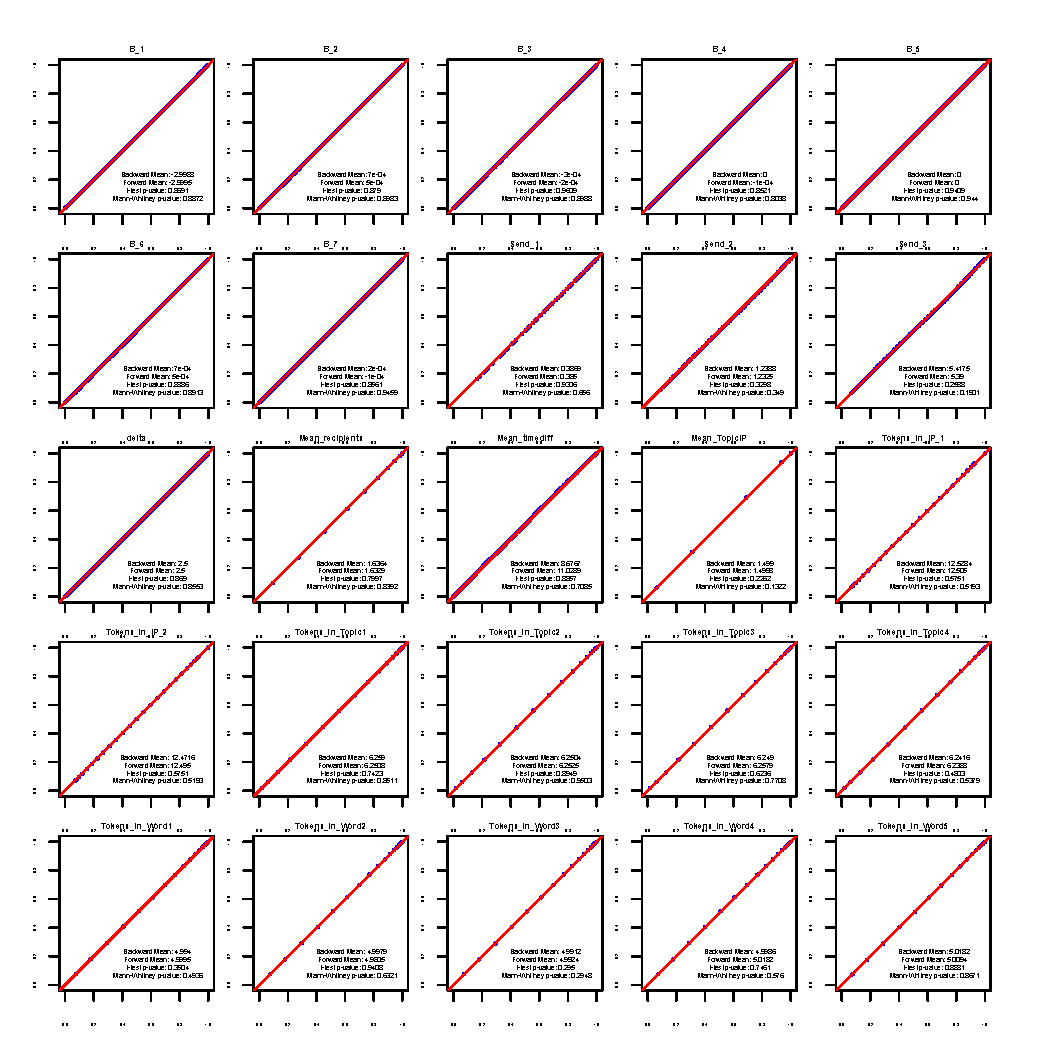
\includegraphics[width=1\textwidth]{plots/Schein.png} 
	\label{fig:PPplot}
	\caption{Probability-Probability plot for the 25 GiR test statistics.}
\end{figure}
 \section{Appliction: North Carolina County Government Email \\ Communication During Hurricane Sandy}  \label{sec: Application to North Carolina email data}
In our application of the IPTM, we use a subset of the North Carolina county government e-mail dataset collected by \citet{ben2017transparency}. This dataset includes internal e-mail corpora covering the inboxes and outboxes of managerial-level employees of North Carolina county governments. Each county corpus covers a three-month span in 2012. The full dataset covers over twenty counties, but we focus on one county, Dare County, for which the time span included a notable national emergency---Hurricane Sandy (October 26, 2012---October 30, 2012). We chose Dare County, (1) in order to see whether and how communication networks surrounding Hurricane Sandy differed from those surrounding other governmental functions, and (2) to limit the scope of this initial application.
  \begin{figure}[ht]
  	\centering
  	     	\includegraphics[width=0.4\textwidth]{plots/Dare.png} 
  	\label{fig:VanceDare}
  	\caption{Geographical location of Dare County in North Carolina}
  \end{figure}
 \subsection{Exploratory Data Analysis} \label{subsec: EDA}
 
Before discussing the IPTM results, we present a set of exploratory analyses in which we examine characteristics of the data that are relevant to the prevalence of Hurricane Sandy in Dare County government email networks. Dare County data spans October 1st to November 30th containing $D=1,456$ emails between $A=27$ actors from 22 departments, and with a vocabulary of size $W=2907$. We ran the exploratory analysis by looking at three different plots---sending and receiving counts, networks, and word counts---to visualize the networks and content of the email data, with emphasis on the changes during hurricane Sandy.
    
In Dare county, we saw considerable change in email sending/receiving behaviors during hurricane Sandy (Figure 4). As the hurricane approaches on October 26th, the manager from the emergency services department sent significantly more emails than before, and at the same time there was dramatic rise in the receiving counts for almost every department. Further analysis demonstrated that emergency services department sent a lot of ``multicast" emails with a large number of receivers during the Sandy period. 
        \begin{figure}[H]
       	\centering
       	\includegraphics[width=0.6\textwidth]{plots/DareSend-1.png} 
       	\includegraphics[width=0.6\textwidth]{plots/DareReceive-1.png} 
       	\label{fig:SendReceiveDare}
       	\caption{The number of emails sent to (upper) and received by (lower) department in Dare County}
       \end{figure}
    
    The network plots in Figure 5 illustrated same patterns we found in Figure 4. Again, the manager from the emergency services department became highly central in the network during the Sandy period, and it maintained this pattern after Sandy. Hurricane related conversations continued after Sandy passed the county, since there remained post-hurricane issues from the damage.
         \begin{figure}[ht]
         	\centering
         	\includegraphics[width=0.75\textwidth]{plots/DareNetwork-1.png} 
         	\label{fig:NetworkDare}
         	\caption{Network plot for three time windows: before Sandy (October 1---October 18), during Sandy (October 19---November 2), and after Sandy (November 3---November 30), in Dare County}
         \end{figure}
         
Figure 6 reflects the hurricane's effects on email exchanges as well, and it matches our interpretations from the network aspects. Usage of the two words, `hurricane' and `Sandy', exploded starting a few days before Sandy arrived in Dare County, and multiple emails used the words again in November, implying the continuous discussions on hurricane-related topics.
            \begin{figure}[ht]
            	\centering
            	\includegraphics[width=0.55\textwidth]{plots/DareWord-1.png}  
            	\label{fig:WordDare}
            	\caption{Frequency plot counting how many times the word `hurricane' and `sandy' appeared}
            \end{figure}
   
  Based on this preliminary exploration, we see that Sandy received significant attention in Dare County. However, this basic descriptive finding does not shed light on whether the network structure of communication surrounding Sandy differed from the typical communication patterns. 
   \subsection{IPTM Results} \label{subsec: IPTM results}
   
   In this section we present the IPTM results. Researchers who use the IPTM can test hypotheses regarding network structure, which is a common---perhaps the most common---use of ERGM-stye models for networks. However, with the IPTM those hypotheses can be conditioned on the content area of communication. To provide an example, we articulate expectations regarding the content-conditional structural properties of the county government email networks. Information diffuses more efficiently in networks characterized by a lack of loops \citep{lin2010measuring,iribarren2011branching} and closed triangles \citep{roca2010topological,tadic2004information}. Assuming that the county governments' internal communication networks are characterized by efficient communication structure,  we expect to see communication regarding the everyday business of the county characterized by negative reciprocity (i.e., 2-loop) effects, and negative triadic effects. The ``receive'' term captures reciprocity, and triadic effects are captured by 2-send, 2-receive, sibling and cosibling. Reciprocity and closed triangles are, however, common structural properties of social networks. We expect to see communication regarding personal/social matters to be characterized by positive reciprocity and triadic effects. Lastly, we have limited expectations regarding how communication surrounding Hurricane Sandy will be structured. We take an exploratory approach to the question of whether or not discussion surrounding Sandy forms an efficient communication network structure.

For the IPTM application to the Dare County email data we used $C=2$ and $K=20$. We ran the model for $O=100$ outer iterations with hyperparameter optimization steps for $n_1=5$, and the inner iterations for $\mathcal{B}$ and $\delta$ were set as $n_2=5500$ and $n_3 = 550$, respectively. This time, first $500$ and $50$ iterations were discarded as a burn-in for inference on  $\mathcal{B}$ and $\delta$, and every $10^{th}$ samples were taken as a thinning process for $\mathcal{B}$. To present the result, each interaction pattern is summarized with (a) Table 1: the top 15 most likely words to be generated in the topics within the interaction pattern, and (b) Table 2: boxplots visualizing posterior estimates of dynamic network effects $\boldsymbol{b}^{(c)}$ within each interaction pattern.
          	
First, we see significant differences in the contents related to each interaction pattern. Overall, 55.2\% of the words were assigned to the topics in interaction pattern 1, and 44.8\% were assigned to the topics in interaction pattern 2. Table 1 demonstrates 5 examples of topics from each interaction pattern, where each topic is summarized by the top 15 words. Interaction pattern 1 seems to represent topics commonly used by government managers. On the other hand, it is interesting that interaction pattern 2 included several topics (e.g. topic 2 and topic 18) with hurricane related words, such as `storm', `impacts' `damage' and `ocean'. In addition, one more impressive point is that topic 12 contained words related politics or election, e.g. `survey', `parties', and `elections'. In summary, interaction pattern 1 represents usual administrative communications between managers in county government, and interaction pattern 2 to reflects temporary conversations driven by events or emergencies occurring in the county.
          		\begin{table}[ht]
          			\centering
          			\scalebox{0.75}{	 	\begin{tabular}{ |c||c|c|c|c|c|}  
          					\hline
          					\textbf{IP} & \textbf{1} &  \textbf{1} & \textbf{1}  &\textbf{1} &\textbf{1}   \\ \hline\hline
          					\textbf{Topic} & \textbf{3} (0.078)&  \textbf{5} (0.065)& \textbf{19} (0.064) &\textbf{13} (0.057) &\textbf{15} (0.053)  \\ \hline\hline
          					\textbf{Word} 
          					& water & planning &phone &questions &contact\\
          					& relocation & meter & collins & board & info \\
          					& location & room & drive &december & problem\\
          					& hills& asked &marshall & call & release \\
          					& utilities &needed & director & sheets & check \\
          					& mustian & sure & human & agenda & weather \\
          					& hydrant &afternoon &resources & nov & priority \\
          					& department &cheryl & manteo & hope & readings \\
          					& skyco & johnson & phr & item & rodanthe \\
          					& kill & issues & fax & weekly & top \\
          					& devil & case & box & management & collection\\ 
          					& road & letter & timesheets &internet & located \\
          					& lane & antennas & -lsb- & told & health \\
          					& tank & inspection & wanted & care & heads \\
          					& map & keep & touch & comp & ahead\\
          					\hline
          					\hline
          					\textbf{IP} & \textbf{2} &  \textbf{2} & \textbf{2}  &\textbf{2} &\textbf{2}   \\ \hline\hline
          					\textbf{Topic} & \textbf{14} (0.058)&  \textbf{12} (0.047)& \textbf{2} (0.045) &\textbf{6} (0.044) &\textbf{18} (0.036) \\ \hline\hline
          					\textbf{Word}
          					& time & survey &  road & library & status \\
          					& hours & voice & mirlo & week & system \\
          					& leave & copy& storm &  working & area \\
          					& monday & discovery & beach & place & south \\
          					& administrative & regional & high & best & forecast \\
          					& employees & parties & coastal & start & track \\
          					& empoyee & disclosed & impacts & visit & pay \\
          					& work & elections & saturday & year & move \\
          					& day & pin & dot & albemarle & assessment \\
          					& friday & sending & night & librarian & opens \\
          					& october & prior & winds & web & damage\\
          					& storm &editor & hold & learning & well\\
          					& tomorrow & students & bridge & east& ocean\\
          					& hour & cost & expressed & holiday &  operation\\
          					& question & residents & normal & system & addition
          					\\
          					\hline            				
          				\end{tabular}}
          				\label{table:TableDare}
          				\caption{Summary of topic-token assignments from Dare County data: top 15 words assigned to each topic, corresponding to interaction pattern assignments}               			
          			\end{table} 
          			
In the Dare County analysis the two interaction patterns exhibited quite different network effects. The effects in interaction pattern 1 were generally greater in magnitude than those in interaction pattern 2, implying that topics related to interaction pattern 2 are less affected by previous email exchanges than those in interaction pattern 1. Most effects are greater in magnitude for the time interval $[t-24h, t)$ and the effect is diminishing as we move to older time intervals $[t-96h, t-24h)$ and $[t-384h, t-96h)$. On the contrary, the statistic `send' had strongest effect in the time interval farthest in the past $[t-384h, t-96h)$. Furthermore, negative reciprocity, which we noted is expected in an efficient communication network, are found in the `receive' statistics effect (except $[t-96h, t-24h)$), in interaction pattern 1.  Most of the posterior distributions of network effects in interaction pattern 2 are centered close to zero, providing little evidence of complex network dynamics. The differences between interaction patterns can be explained by the content differences conveyed through Table 1. Since interaction pattern 2 consists of highly time-sensitive topics, ties are less likely to be effected by previous interactions.
          	\begin{table}[ht]
          		\centering
          		\begin{tabular}{lll}
          			\includegraphics[width = 0.3\textwidth]{plots/DareIntercept-1.png} &
          			\includegraphics[width = 0.3\textwidth]{plots/DareOutdegree-1.png} &
          			\includegraphics[width = 0.3\textwidth]{plots/DareIndegree-1.png} \\
          			\includegraphics[width = 0.3\textwidth]{plots/DareBSend-1.png} &
          			\includegraphics[width = 0.3\textwidth]{plots/DareBReceive-1.png} &
          			\includegraphics[width = 0.3\textwidth]{plots/Dare2Send-1.png}   \\ 
          			\includegraphics[width = 0.3\textwidth]{plots/Dare2Receive-1.png} &
          			\includegraphics[width = 0.3\textwidth]{plots/DareSibling-1.png} &
          			\includegraphics[width = 0.3\textwidth]{plots/DareCosibling-1.png}   \\         	
          		\end{tabular}
          		\label{fig:DareB}
          		\caption{95\% credible intervals of posterior estimates of the network effects $\boldsymbol{b}^{(c)}$: $c=1$ (red) and $c=2$ (green), using Dare County data}
          	\end{table}
          	
  \section{Document Prediction Experiments} \label{sec:PosteriorPredictive}
 We use a set of posterior predictive experiments, or document-ahead forecasting, to evaluate the performance of the IPTM as compared to alternative parameterizations of the IPTM and alternative modeling approaches via regressions. For a randomly chosen document $D \in \{M,M+1,\hdots, D\}$, we fit the IPTM to the corpus consisting of the first $d = \{1,\hdots,D-1\}$ documents, then use the inferred posterior distributions to generate a distribution of predicted tie data for document $D$ conditional on the content in document $D$, $\boldsymbol{w}^{(D)}$.  A reasonable choice for $M$ would be $D/2$, to assure a sufficient size training set for the first document in the test set. The variables that need to be sampled are the tie data ($i_o^{(D)}, J_o^{(D)}, t_o^{(D)}$), and we would compare the simulated ones to the observed data. Detailed pseudocode for generating predicted tie data using the IPTM is demonstrated in Appendix \ref{subsubsec: IPTM PPE}.

\subsection{Comparison Models}\label{subsec:ComparisonModels}
We first compare the ability of the IPTM in predicting tie data to that of the reduced parameterization of the IPTM. Specifically, by setting the number of interaction pattern $C = 1$ (i.e. $\{p_c^{d}\}_{d=1}^D = 1$), the IPTM reduces to pure network model which disregards the content reflection on network dynamics. However, this reduced version of the model still is innovative network model in that we jointly make inference on sender, receiver, and timestamp of the document. There exists numerous network modeling approaches in the literature, however, we are unaware of a model that can be used to jointly predict the sender, receivers, and timing of an e-mail/document conditional upon the interaction history. Therefore, the two main goals of this ablation study are 1) to test whether the reduced model itself serves as a novel network model with good predictive performance, and 2) to test whether including content information via interaction pattern provides additional advantage on document-ahead forecasting for tie data.

Next, we compare the IPTM to the comparative model that is built upon two regression models, in order to test if the IPTM or the ablated version of IPTM have any benefit over other existing models. To build an alternative modeling approach, we combine established existing models to make comparable predictions using the same inputs. The objective underlying our selection and use of comparison models is to evaluate the performance gains from jointly inferring the parameters that govern the generation of tie data---senders, receivers, and timing. Several models exist that could be used to model any of these three data types individually, but, to our knowledge, the literature does not offer any models that can be used to jointly generate all three types of tie data integrated into the IPTM. We train two separate models to use in predicting document $D$ recipients, sender, and timing, respectively. These models are selected to closely mirror the structure of the corresponding components of the IPTM. In each model the documents used for training include documents $1$ through $D-1$. The model of recipients will be a logistic regression model in which the dependent variable is the observed value of $J^{(d)}_{ij}$, where $i$ indexes the observed sender, $i_o^{(d)}$. The network statistics, $\boldsymbol{x}^{(c)}_t(i, j)$, will be used as the covariates, with all $c=1$ (i.e., all past interactions are within the same single interaction pattern in the comparison models). Specifically, the model used for predicting recipients of document $D$ will have the form 
\begin{equation}
P(J^{(D)}_{ij}=1)=\frac{1}{1+\exp\left(-(b_0 +\boldsymbol{b}^T\boldsymbol{x}_t(i, j))\right)}.
\label{eqn:predrec}
\end{equation}
The model of when an email was sent is an exponential regression model in which the dependent variable is $t_i^{(D)}$. The single covariate in this model, assumed to have a coefficient of 1, is $\lambda_{iJ_i}^{(D)}(t)$, which is defined in Equation (\ref{alg:multicastlambda}). We estimate an intercept term in this regression model in order to calibrate the scale of the model. Specifically, the probability density function of the model for the timing of the email is given by
\begin{equation}
f(t_i^{(D)},\lambda_{iJ_i}^{(D)}(t),\eta) = \eta\lambda_{iJ_i}^{(D)}(t)\exp(- \eta\lambda_{iJ_i}^{(D)}(t)t_i^{(D)}),
\label{eqn:predtime}
\end{equation}
where $\ln(\eta)$ is the intercept that calibrates the scale of the exponential distribution. The predicted sender of document $D$ is determined by simulating $t_i^{(D)}$ for each $i$, and selecting the $i$ that corresponds to the minimum value of $t_i^{(D)}$. The minimum value of $t_i^{(D)}$ is the predicted timing for document $D$, i.e. $t_o^{(D)}$, and similarly as the IPTM, the minimum time chooses the sender and recipient of the document D, i.e. $i_o^{(D)}$ and $J_o^{(D)}$. See Appendix \ref{subsubsec: Regression PPE} for pseudocode.
\subsection{Predictive Experiment Results}
To verify that our model is applicable beyond the Dare County email data, we also performed the posterior predictive experiments using the Enron email data set ---the most widely studied email data set. For this data set, we only included emails between actors who sent over 100 emails, and actors who received over 100 emails from the chosen senders. E-mails that were not sent to at least one other active actor were discarded, and also preprocessed to remove any stop words, URLs, quoted text, and signatures. These steps resulted in a total of 3,925 emails involving 33 actors. 

For both data sets, Dare County and Enron, we randomly selected 200 documents from the later half of the corpus and generated 100 samples of predicted tie data for every document $D$ by running Algorithm \ref{alg:IPTMPPE} and Algorithm \ref{alg:docpredict} ($O = 10$ and $R = 50$) with some burn-ins and thinnings ($b = 10$ and $q = 4$). Due to computational burden, we used the reduced set of network statistics (``intercept" and ``dyadic") for Enron, while we used full set of network statistics (``intercept" and ``dyadic", ``degree", ``triadic"). Moreover, we ran the same predictive experiments with 21 unique combinations of the number of interaction patterns ($C = 1, 2, 3$) and the number of topics ($K = 2, 5, 10, 25, 50, 75, 100$) as a grid-search based hyperparameter selection process. After choosing the best-performing hyperparameter combinations from the prediction results of earlier 150 documents, we then use the prediction results of the rest 50 documents to compare the IPTM and these predictions in terms of classification accuracy in predicting senders and receivers, as well as mean squared error in predicting document timing. Figure 7 presents the $F_1$ scores on sender predictions, multiclass version of the area under the ROC curve (AUC) measure \citep{hand2001simple} on receiver predictions, and mean squared error (MSE) on time predictions for each document we predicted, all averaged over 100 samples. 

\textbf{Note: Plots to be updated when we get further results}
\begin{figure}[ht]
	\centering
	\includegraphics[width=1\textwidth]{plots/Dare_PPE.pdf}  
		\includegraphics[width=1\textwidth]{plots/Enron_PPE.pdf}  
	\label{fig:PPE}
	\caption{Average AUC, F1 score, MSE for the Dare County email network (upper) and the Enron data set (lower).}
\end{figure}

\section{Topic Coherence} \label{sec:topiccoherence}
Topic coherence metrics \cite{mimno2011optimizing} are often used to evaluate the semantic coherence in topic models. In order to test whether the IPTM's incorporation of network properties improves or impairs the ability of modeling text, we compared the coherence of topics inferred using our model with the coherence of topics inferred using the latent dirichlet allocation (LDA). Instead of re-fit the data using standard LDA algorithms, we used the topic assignments from the IPTM with $C=1$, which simply makes the IPTM reduced to LDA in terms of topic assignments by unlinking the text and networks (same analogy as ablation study in Section \ref{subsec:ComparisonModels}). For each model, we varied the number of topics from 1 to 100 and drew five samples from the joint posterior distribution over the unobserved random variables in that model. We evaluated the topics resulting from each sample and averaged over the five samples, where the result is shown in Figure \ref{fig:Daretopic}. Our model was not significantly different from LDA in terms of topic coherence, for any choice of the number of topics. This result, when combined with the results in Section 7, demonstrates that our model can achieve state-of-the-art predictive performance while producing coherent topics. 

\textbf{Note: Plots to be updated when we get further results, including Enron's.}
\begin{figure}[ht]
	\centering
	\includegraphics[width=0.49\textwidth]{plots/Dare_topic.pdf}  
	\label{fig:Daretopic}
	\caption{Average topic coherence scores for the Dare County email network (left) and the Enron data set (right).}
\end{figure}


\section{Posterior Predictive Checks}

We finally perform posterior predictive checks \cite{rubin1984bayesianly} in order to evaluate the appropriateness of the model specification for Dare county. If the model is appropriate, the observed data should not be an outlier with respect to distributions of new data drawn from the posterior predictive distribution. To draw these comparisons, we first consider how to draw from the posterior predictive distribution. We produce a sample from the posterior predictive distribution by drawing new data conditional upon the parameters inferred in a single draw from the posterior distribution of the parameters, repeated over many draws from the posterior distribution. 

Formally, we generate new data, which we denote ($\mathcal{I}_{\mbox{o}}^*, \mathcal{J}_{\mbox{o}}^*, \mathcal{T}_{\mbox{o}}^*,\mathcal{W}^*$), conditional upon a set of inferred parameter values from
\begin{equation}
P(\mathcal{I}_{\mbox{o}}^*, \mathcal{J}_{\mbox{o}}^*, \mathcal{T}_{\mbox{o}}^*,\mathcal{W}^* |\mathcal{Z}, \mathcal{C}, \mathcal{B}, \delta,\boldsymbol{u}, \alpha, \boldsymbol{m}, \mu_{\boldsymbol{b}}, \Sigma_{\boldsymbol{b}}, \mu_\delta, \sigma^2_\delta),
\label{eqn:backwardssample}
\end{equation}
and the pseudocode for generating new sets of data is given by Appendix \ref{subsec:Details on PPC}.

 We use this posterior predictive checking to assess the extent to which our model is a ``good fit" for the Dare County email network. For the test of goodness-of-fit in terms of network dynamics, we defined multiple network statistics that summarize meaningful aspects of Dare County data: indegree distribution for sender activities, outdegree distribution for receiver activities, document time-increment distributions, multicast (number of receivers) distribution, the edgewise shared partner distribution, and the geodesic distance distribution. For content-wise goodness-of-fit, we employed mutual information (MI) in \cite{mimno2011bayesian}, which is often used to evaluate ``bag of words" model assumptions. We then generated 1,000 synthetic networks and texts from the posterior predictive distribution implied by the IPTM and Dare County email data.
We applied each discrepancy function to each synthetic network to yield the distributions over the values of the six network statistics and MI. If the IPTM is a suitable model for Dare County data, these distributions should be centered around the values of the corresponding discrepancy functions (except MI) when computed using the observed data.

\textbf{Note: Plots and analysis to be added when we get the results}

\section{Conclusion} 
The IPTM is, to our knowledge, the first model to be capable of jointly modeling sender, receivers, time and contents in time stamped text valued networks. The IPTM incorporates innovative components, including the modeling of multicast tie formation and the conditioning of ERGM style network generative features on topic-based content. The application to North Carolina county government email data demonstrates, among other capabilities, the effectiveness at the IPTM in separating out both the content and relational structure underlying the normal day-to-day function of an organization and the management of a highly time-sensitive event---Hurricane Sandy. The IPTM is applicable to a variety of networks in which ties are attributed with textual documents. These include, for example, economic sanctions sent between countries and legislation attributed with sponsors and co-sponsors. 
 \clearpage
\bibliographystyle{apalike}
\bibliography{IPTM}
\newpage
\appendix
 \section*{Appendix}
 \renewcommand{\thesubsection}{\Alph{subsection}}
   	 \subsection{Normalizing constant of non-empty Gibbs measure}\label{subsec: non-empty Gibbs measure}
  	 In Section \ref{subsec: Tie Generating Process}, we define the non-empty Gibbs measure such that 
 the probability of sender $i$ selecting the binary receiver vector of length $(A-1)$, $J_i^{(d)}$ is given by
  	 \begin{equation*} \text{P}(J_i^{(d)}) = \frac{1}{Z(\delta,\mbox{log}(\lambda_i^{(d)}))} \exp\Big\{ \mbox{log}\big(\text{I}(\lVert J_i^{(d)} \rVert_1 > 0)\big) + \sum_{j \in \mathcal{A}_{\backslash i}} (\delta+\mbox{log}(\lambda_{ij}^{(d)}))J_{ij}^{(d)} \Big\}.
  	 \end{equation*}
  	 	 To use this distribution efficiently, we derive a closed-form expression for $Z(\delta,\mbox{log}(\lambda_{i}^{(d)}))$ that does not require brute-force summation over the support of $J_i^{(d)}$. We recognize that if $J_i^{(d)}$ were drawn via independent Bernoulli distributions in which P($J_{ij}^{(d)}$=1) was given by logit$(\delta+\lambda_{ij}^{(d)})$, then \begin{equation*}\text{P}(J_i^{(d)}) \propto \exp\Big\{  \sum_{j \in \mathcal{A}_{\backslash i}} (\delta+\mbox{log}(\lambda_{ij}^{(d)}))J_{ij}^{(d)}\Big\}.  	 \end{equation*}
  	 	  This is straightforward to verify by looking at 
  	 	  \begin{equation*}
  	 	  \begin{aligned}\text{P}(J_{ij}^{(d)}=1|J_{i,-j})&=\frac{ \exp{(\delta+\mbox{log}(\lambda_{ij}^{(d)}))}\exp\Big\{ \sum_{h\neq i,j} (\delta+\mbox{log}(\lambda_{ih}^{(d)}))J_{ih}^{(d)} \Big\}}{\exp{(\delta+\mbox{log}(\lambda_{ij}^{(d)}))}\exp\Big\{   \sum_{h\neq i,j} (\delta+\mbox{log}(\lambda_{ih}^{(d)}))J_{ih}^{(d)} \Big\}+ \exp{(0)}\exp\Big\{ \sum_{h\neq i,j} (\delta+\mbox{log}(\lambda_{ih}^{(d)}))J_{ih}^{(d)} \Big\}},\\
  	 	  &=\frac{ \exp{(\delta+\mbox{log}(\lambda_{ij}^{(d)}))}}{\exp{(\delta+\mbox{log}(\lambda_{ij}^{(d)}))} + 1}.\end{aligned}\end{equation*}
  	 	  We denote the logistic-Bernoulli normalizing constant as $Z^{l}(\delta,\lambda_i^{(d)})$, which is defined as 
  	 	  \begin{equation*}
  	 	  Z^{l}(\delta,\mbox{log}(\lambda_{i}^{(d)}))=\sum_{J_i \in [0,1]^{(A-1)}} \exp\Big\{\sum_{j\neq i} (\delta+\mbox{log}(\lambda_{ij}^{(d)}))J_{ij}^{(d)} \Big\}.
  	 	  \end{equation*}
  	 
  	 Now, since 
  	\begin{equation*}
  	\exp\Big\{ \mbox{log}\big(\text{I}(\lVert J^{(d)} \rVert_1> 0 )\big) + \sum_{j \in \mathcal{A}_{\backslash i}} (\delta+\mbox{log}(\lambda_{ij}^{(d)}))J_{ij}^{(d)} \Big\}= \exp\Big\{ \sum_{j \in \mathcal{A}_{\backslash i}} (\delta+\mbox{log}(\lambda_{ij}^{(d)}))J_{ij}^{(d)} \Big\},
  	\end{equation*} except when $\lVert J^{(d)} \rVert_1=0$, in which case the left-hand side 
  	\begin{equation*}
\exp\Big\{ \mbox{log}\big(\text{I}(\lVert J^{(d)} \rVert_1> 0 )\big) + \sum_{j \in \mathcal{A}_{\backslash i}} (\delta+\mbox{log}(\lambda_{ij}^{(d)}))J_{ij}^{(d)} \Big\}= 0.  	
\end{equation*}
 As such, we note that 
 \begin{equation*}
 \begin{aligned}
Z(\delta,\mbox{log}(\lambda_{i}^{(d)}))& = Z^{l}(\delta,\mbox{log}(\lambda_{i}^{(d)})) -  \exp\Big\{ \sum\limits_{\substack{j \in \mathcal{A}_{\backslash i}, J^{(d)}_{ij}=0}} (\delta+\mbox{log}(\lambda_{ij}^{(d)}))J_{ij}^{(d)} \Big\}
\\& = Z^{l}(\delta,\mbox{log}(\lambda_{i}^{(d)})) -  1.
\end{aligned}
 \end{equation*}
   We can therefore derive a closed form expression for $Z(\delta,\mbox{log}(\lambda_{i}^{(d)}))$ via a closed form expression for $Z^{l}(\delta,\mbox{log}(\lambda_{i}^{(d)}))$. This can be done by looking at the probability of the zero vector under the logistic-Bernoulli model:
   \begin{equation*}
   \begin{aligned}
\frac{\exp\Big\{\sum_{j\neq i, J^{(d)}_{ij}=0} (\delta+\mbox{log}(\lambda_{ij}^{(d)}))J_{ij}^{(d)} \Big\}}{Z^{l}(\delta,\mbox{log}(\lambda_{ij}^{(d)}))} &= \prod_{j \in \mathcal{A}_{\backslash i} }   \frac{ \exp\{-(\delta+\mbox{log}(\lambda_{ij}^{(d)}))\}}{\exp\{-(\delta+\mbox{log}(\lambda_{ij}^{(d)}))\} + 1},\\
Z^{l}(\delta,\mbox{log}(\lambda_{ij}^{(d)})) &= \frac{1}{\prod_{j \in \mathcal{A}_{\backslash i}}   \frac{ \exp\{-(\delta+\mbox{log}(\lambda_{ij}^{(d)}))\}}{\exp\{-(\delta+\mbox{log}(\lambda_{ij}^{(d)}))\} + 1}}.
  	 \end{aligned}  
  	 \end{equation*}
  	 The closed form expression for the normalizing constant under the non-empty Gibbs measure is therefore    \begin{equation*}
  	 \begin{aligned}Z(\delta,\lambda_i^{(d)}) = \Big(\prod_{j \in \mathcal{A}_{\backslash i}} \Big(\mbox{exp}\{\delta+\mbox{log}(\lambda_{ij}^{(d)})\} + 1\Big)\Big)-1.
  	  \end{aligned}  
  	  \end{equation*}
  	  \subsection{Sampling Equations}\label{subsec:Sampling Equations}
  	     \subsubsection{Joint distribution of latent and observed tie variables}\label{subsubsec:Joint distribution of Tie}
  	       As mentioned earlier in Section \ref{subsec: Tie Generating Process}, we use data augmentation in the tie generating process. Since we should include both the observed and augmented data to make inferences on the related latent variables, the derivation steps for the contribution of tie data is not as smiple as other variables. Therefore, here we provide the detailed derivation steps for the last term of joint posterior distribution in Equation (\ref{alg:jointposterior}), starting from the likelihood before integriting out the latent time $\mathcal{T}_{\mbox{a}}$: 
  	       \begin{equation}
  	       \begin{aligned}
  	       &P(\mathcal{J}_{\mbox{a}}, \mathcal{T}_{\mbox{a}},\mathcal{I}_{\mbox{o}}, \mathcal{J}_{\mbox{o}}, \mathcal{T}_{\mbox{o}} |\mathcal{Z}, \mathcal{C}, \mathcal{B}, \delta)
  	       \\& \propto P(\mathcal{J}^{(1)}_{\mbox{a}}, ...,\mathcal{J}^{(D)}_{\mbox{a}}, \mathcal{T}^{(1)}_{\mbox{a}},...,\mathcal{T}^{(D)}_{\mbox{a}}, i^{(1)}_{\mbox{o}},...,i^{(D)}_{\mbox{o}}, J^{(1)}_{\mbox{o}},...,J^{(D)}_{\mbox{o}}, t^{(1)}_{\mbox{o}},...,t^{(D)}_{\mbox{o}} |\mathcal{Z}, \mathcal{C}, \mathcal{B}, \delta)
  	       \\& \propto P(\mathcal{J}^{(D)}_{\mbox{a}}, \mathcal{T}^{(D)}_{\mbox{a}}, i^{(D)}_{\mbox{o}}, J^{(D)}_{\mbox{o}}, t^{(D)}_{\mbox{o}} |\mathcal{I}^{(<D)}_{\mbox{o}}, \mathcal{J}^{(<D)}_{\mbox{o}}, \mathcal{T}^{(<D)}_{\mbox{o}},\mathcal{Z}, \mathcal{C}, \mathcal{B}, \delta).
  	       \end{aligned}
  	       \end{equation}
  	       Note that the joint likelihood of document $d=1,...,D$ is proportional to the likelihood of $D^{th}$ document, since the documents are not independent; all tie variables in $D^{th}$ are conditioned on the earlier documents $(<D)$ via network covariates $\boldsymbol{x}$ or past interaction history. \\ \newline
  	       Now we tackle the problem of evaluating the last line of Equation (9) by deriving the likelihood for $d^{th}$ document, $P(\mathcal{J}^{(d)}_{\mbox{a}}, \mathcal{T}^{(d)}_{\mbox{a}}, i^{(d)}_{\mbox{o}}, J^{(d)}_{\mbox{o}}, t^{(d)}_{\mbox{o}} |\mathcal{I}^{(<d)}_{\mbox{o}}, \mathcal{J}^{(<d)}_{\mbox{o}}, \mathcal{T}^{(<d)}_{\mbox{o}}, \mathcal{Z}, \mathcal{C}, \mathcal{B}, \delta)$. There are three steps involved. First is the generation of the latent receivers $J_i$ for each $i$; second is the generation of the observed time increment $\Delta T^{(d)} = t^{(d)} - t^{(d-1)}$ from the observed sender-receiver pairs ($i^{(d)}_{\mbox{o}}, J^{(d)}_{\mbox{o}}$); and the last part is the simultaneous selection process of the observed sender, receivers, and timestamp, implying that the latent time increments generated from the latent sender-receiver pairs were greater than the observed time increment. Reflecting the three steps, the joint distribution is:\\
  	       \begin{equation}
  	       \begin{aligned}
  	       &P(\mathcal{J}^{(d)}_{\mbox{a}}, \mathcal{T}^{(d)}_{\mbox{a}}, i^{(d)}_{\mbox{o}}, J^{(d)}_{\mbox{o}}, t^{(d)}_{\mbox{o}} |\mathcal{I}^{(<d)}_{\mbox{o}}, \mathcal{J}^{(<d)}_{\mbox{o}}, \mathcal{T}^{(<d)}_{\mbox{o}}, \mathcal{Z}, \mathcal{C}, \mathcal{B}, \delta)\\&=P\Big(\mbox{latent receivers generation}\Big) \times P\Big(\mbox{latent time generation}\Big)\times P\Big(\mbox{choose the observed}\Big) \\&
  	       =\prod_{i\in \mathcal{A}}\Big(J_{i}^{(d)}\sim \mbox{Gibbs measure}(\{\lambda_{ij}^{(d)}\}_{j=1}^A,\delta)\Big) \times \prod_{i\in \mathcal{A}}\Big(\Delta T^{(d)}_{iJ_i}\sim\mbox{Exp}(\lambda^{(d)}_{iJ_i})\Big) \times \prod_{i\in \mathcal{A}_{\backslash i_o^{(d)}}} P\Big(\Delta T^{(d)}_{i{J_i}} > \Delta T_{i_{o}^{(d)}{J_{o}^{(d)}}}\Big)\\&
  	       =\Big(\prod_{i\in \mathcal{A}}\frac{1}{Z(\delta,\mbox{log}(\lambda_i^{(d)}))} \exp\Big\{ \mbox{log}\big(\text{I}( \sum_{j \in \mathcal{A}_{\backslash i}} J^{(d)}_{ij} > 0 )\big) + \sum_{j \in \mathcal{A}_{\backslash i}} (\delta+\mbox{log}(\lambda_{ij}^{(d)}))J_{ij}^{(d)} \Big\}\Big)\\&\quad\quad\quad\quad\quad\quad\quad\quad\quad\quad\quad\quad\quad\quad\quad\quad\quad\quad\times \Big(\prod_{i \in\mathcal{A}}\lambda^{(d)}_{iJ_i}e^{-\Delta T^{(d)}_{iJ_i}\lambda^{(d)}_{iJ_i}}\Big)\times \Big( \prod_{i\in \mathcal{A}_{\backslash i_o^{(d)}}} e^{-\Delta T^{(d)}_{i_o^{(d)}J_o^{(d)}}\lambda^{(d)}_{iJ^{(d)}_{i}}}\Big)
  	       \\&
  	       \propto \Big(\prod_{i\in \mathcal{A}}\frac{1}{\Big(\prod_{j \in \mathcal{A}_{\backslash i}} \Big(\mbox{exp}\{\delta+\mbox{log}(\lambda_{ij}^{(d)})\} + 1\Big)\Big)-1}\exp\Big\{ \sum_{j \in \mathcal{A}_{\backslash i}} (\delta+\mbox{log}(\lambda_{ij}^{(d)}))J_{ij}^{(d)} \Big\}\Big)\\&\quad\quad\quad\quad\quad\quad\quad\quad\quad\quad\quad\quad\quad\quad\quad\quad\quad\quad\times\Big(\lambda^{(d)}_{i_o^{(d)}J_o^{(d)}}e^{-\Delta T^{(d)}_{i_o^{(d)}J_o^{(d)}}\lambda^{(d)}_{i_o^{(d)}J_o^{(d)}}}\Big)	\times \Big( \prod_{i\in \mathcal{A}_{\backslash i_o^{(d)}}} \lambda^{(d)}_{iJ_i}e^{-(\Delta T^{(d)}_{iJ_i} + \Delta T^{(d)}_{i_o^{(d)}J_o^{(d)}})\lambda^{(d)}_{iJ_i}}\Big),
  	       \end{aligned}
  	       \end{equation}
  	       We simplify further by integreting out the latent time $\mathcal{T}^{(d)}_{\mbox{a}}=\{\Delta T^{(d)}_{iJ_i}\}_{i \in \mathcal{A}_{\backslash i_o^{(d)}}}$ in the last term:
  	       \begin{equation}
  	       \begin{aligned}
  	       &\int_{0}^\infty\cdots\int_{0}^\infty \Big(\prod_{i\in \mathcal{A}_{\backslash i_o^{(d)}}} \lambda^{(d)}_{iJ_i}e^{-(\Delta T^{(d)}_{iJ_i} + \Delta T^{(d)}_{i_o^{(d)}J_o^{(d)}})\lambda^{(d)}_{iJ_i}} \Big)d\Delta T^{(d)}_{1J_1}\cdots d\Delta T^{(d)}_{AJ_A}\\&
  	       = \prod_{i\in \mathcal{A}_{\backslash i_o^{(d)}}} e^{- \Delta T^{(d)}_{i_o^{(d)}J_o^{(d)}}\lambda^{(d)}_{iJ_i}} \Big(\int_{0}^\infty \lambda^{(d)}_{iJ_i}e^{-\Delta T^{(d)}_{iJ_i} \lambda^{(d)}_{iJ_i}}  d\Delta T^{(d)}_{iJ_i}\Big)
  	       \\& =\prod_{i\in \mathcal{A}_{\backslash i_o^{(d)}}} e^{- \Delta T^{(d)}_{i_o^{(d)}J_o^{(d)}}\lambda^{(d)}_{iJ_i}} \Big(\Big [ - e^{-\Delta T^{(d)}_{iJ_i} \lambda^{(d)}_{iJ_i}}\Big]_{\Delta T^{(d)}_{iJ_i}  = 0} ^{\infty}\Big)
  	       \\& = e^{- \Delta T^{(d)}_{i_o^{(d)}J_o^{(d)}}\sum_{i\in \mathcal{A}_{\backslash i_o^{(d)}}}\lambda^{(d)}_{iJ_i}},
  	       \end{aligned}
  	       \end{equation}
  	       where $\Delta T^{(d)}_{i_o^{(d)}J_o^{(d)}}$ is the observed time difference between $d^{th}$ and $(d-1)^{th}$ document. Therefore, we simplify Equation (13) as below:
  	       \begin{equation}
  	       \begin{aligned}
  	       &P(\mathcal{J}^{(d)}_{\mbox{a}}, i^{(d)}_{\mbox{o}}, J^{(d)}_{\mbox{o}}, t^{(d)}_{\mbox{o}} |\mathcal{I}^{(<d)}_{\mbox{o}}, \mathcal{J}^{(<d)}_{\mbox{o}}, \mathcal{T}^{(<d)}_{\mbox{o}}, \mathcal{Z}, \mathcal{C}, \mathcal{B}, \delta)\\&\propto \Big(\prod_{i\in \mathcal{A}}\frac{1}{\Big(\prod_{j \in \mathcal{A}_{\backslash i}} \Big(\mbox{exp}\{\delta+\mbox{log}(\lambda_{ij}^{(d)})\} + 1\Big)\Big)-1}\exp\Big\{ \sum_{j \in \mathcal{A}_{\backslash i}} (\delta+\mbox{log}(\lambda_{ij}^{(d)}))J_{ij}^{(d)} \Big\}\Big)\\&\quad\quad\quad\quad\quad\quad\quad\quad\quad\quad\quad\quad\quad\quad\quad\quad\quad\quad\times \Big(\lambda^{(d)}_{i_o^{(d)}J_{o}^{(d)}}\Big)\times\Big( e^{-\Delta T^{(d)}_{i_o^{(d)}J_o^{(d)}}\sum\limits_{i\in \mathcal{A}}\lambda^{(d)}_{iJ^{(d)}_{i}}}\Big),
  	       \end{aligned}
  	       \end{equation}
  	       where this joint distribution can be interpreted as `probability of latent and observed edges from non-empty Gibbs measure $\times$ probability of the observed time-increment comes from Exponential distribution $\times$ probability of all latent time greater than the observed time, given that the latent time-increments also come from Exponential distribution.'
  	       Finally for implementation, we need to compute these equations in log space to prevent underflow:
  	       \begin{equation}
  	       \begin{aligned}
  	       &\mbox{log}\Big(P(\mathcal{J}^{(d)}_{\mbox{a}}, i^{(d)}_{\mbox{o}}, J^{(d)}_{\mbox{o}}, t^{(d)}_{\mbox{o}} |\mathcal{I}^{(<d)}_{\mbox{o}}, \mathcal{J}^{(<d)}_{\mbox{o}}, \mathcal{T}^{(<d)}_{\mbox{o}}, \mathcal{Z}, \mathcal{C}, \mathcal{B},  \delta)\Big)\\&\propto \Big(\sum_{i\in \mathcal{A}}\Big(-\log\Big(\Big(\prod_{j \in \mathcal{A}_{\backslash i}} \Big(\mbox{exp}\{\delta+\mbox{log}(\lambda_{ij}^{(d)})\} + 1\Big)\Big)-1\Big) + \sum_{j \in \mathcal{A}_{\backslash i}} (\delta+\mbox{log}(\lambda_{ij}^{(d)}))J_{ij}^{(d)}\Big)\Big)\\&\quad\quad\quad\quad\quad\quad\quad\quad\quad\quad\quad\quad\quad\quad\quad\quad\quad\quad +  \Big(\mbox{log}(\lambda^{(d)}_{i_o^{(d)}J_o^{(d)}})\Big){ - \Big(\Delta T^{(d)}_{i_o^{(d)}J_o^{(d)}}\sum\limits_{i \in \mathcal{A}}\lambda^{(d)}_{i{J_i^{(d)}}}}\Big).
  	       \end{aligned}
  	       \end{equation}
   \subsubsection{Resampling $\mathcal{J}_{\mbox{a}}$} \label{subsec: Data augmentation}
   First of all, for each document $d$, we sample the latent sender-receiver(s) pairs as in pseudocode (Algorithm 6). That is, given the observed sender of the document $i_o^{(d)}$, we sample the latent receivers for each sender $i \in \mathcal{A}_{\backslash i_o^{(d)}}$. Here we illustrate how each sender-receiver pair in the document $d$ is updated.\\\newline
   Define ${\mathcal{J}}^{(d)}_{i}$ be the $(A-1)$ length random vector of indicators with its realization being $J^{(d)}_{i}$, representing the latent receivers corresponding to the sender $i$ in the document $d$. For each latnet sender $i$, we are going to resample ${J}^{(d)}_{ij}$, which is the $j^{th}$ element of the receiver vector ${J}^{(d)}_{i}$, one at a time with random order. The full conditional probability of ${J}^{(d)}_{ij}$ is:
   \begin{equation}
   \begin{aligned}
   & P(\mathcal{J}^{(d)}_{ij} = {J}^{(d)}_{ij}|\mathcal{J}^{(d)}_{i\backslash j}, \mathcal{Z}, \mathcal{C},   \mathcal{B}, \delta, \mathcal{W},  \mathcal{J}_{\mbox{a}, -i}, \mathcal{I}_{\mbox{o}}, \mathcal{J}_{\mbox{o}}, \mathcal{T}_{\mbox{o}}, \beta, \boldsymbol{u}, \alpha, \boldsymbol{m},  \mu_{\boldsymbol{b}}, \Sigma_{\boldsymbol{b}}, \mu_\delta, \sigma^2_\delta),
   \end{aligned}
   \end{equation}
   which we can drop some independent terms and move to 
   \begin{equation}
   \begin{aligned}
   &P(\mathcal{J}^{(d)}_{ij} = {J}^{(d)}_{ij}|\mathcal{J}^{(d)}_{i\backslash j}, i^{(d)}_{\mbox{o}}, J^{(d)}_{\mbox{o}}, t^{(d)}_{\mbox{o}}, \mathcal{I}^{(<d)}_{\mbox{o}}, \mathcal{J}^{(<d)}_{\mbox{o}}, \mathcal{T}^{(<d)}_{\mbox{o}}, \mathcal{Z}, \mathcal{C}, \mathcal{B}, \delta)\\&\propto P(\mathcal{J}^{(d)}_{ij} ={J}^{(d)}_{ij}, \mathcal{J}^{(d)}_{i\backslash j}, i^{(d)}_{\mbox{o}}, J^{(d)}_{\mbox{o}}, t^{(d)}_{\mbox{o}}| \mathcal{I}^{(<d)}_{\mbox{o}}, \mathcal{J}^{(<d)}_{\mbox{o}}, \mathcal{T}^{(<d)}_{\mbox{o}}, \mathcal{Z}, \mathcal{C}, \mathcal{B}, \delta)
   \\&\propto\Big( \frac{1}{\Big(\prod_{j \in \mathcal{A}_{\backslash i}} \Big(\mbox{exp}\{\delta+\mbox{log}(\lambda_{ij}^{(d)})\} + 1\Big)\Big)-1}\exp\Big\{\mbox{log}\big(\text{I}( \sum_{j \in \mathcal{A}_{\backslash i}} J^{(d)}_{ij} > 0 )\big) +\sum_{j \in \mathcal{A}_{\backslash i}} (\delta+\mbox{log}(\lambda_{ij}^{(d)}))J_{ij}^{(d)} \Big\}\Big)\\&\quad\quad\quad\quad\quad\quad\quad\quad\quad\quad\quad\quad\quad\quad\quad\quad\quad\quad\quad\quad\quad\times \Big(\lambda^{(d)}_{i_o^{(d)}J_{o}^{(d)}}\Big)\times \Big(e^{-\Delta T^{(d)}_{i_o^{(d)}J_o^{(d)}}\lambda^{(d)}_{iJ^{(d)}_{i}}}\Big)
   \\& \propto \Big(\exp\Big\{\mbox{log}\big(\text{I}( \lVert J_i^{(d)} \rVert_1 > 0 )\big) +\sum_{j \in \mathcal{A}_{\backslash i}} (\delta+\mbox{log}(\lambda_{ij}^{(d)}))J_{ij}^{(d)} \Big\}\Big)\times \Big(e^{-\Delta T^{(d)}_{i_o^{(d)}J_o^{(d)}}\lambda^{(d)}_{iJ^{(d)}_{i}}}\Big),
   \end{aligned}
   \end{equation}
   where we replace typical use of $(-d)$ to $(<d)$ on the right hand side, due to the fact that $d^{(th)}$ document only depends on the past documents. The last line of Equation (18) is obtained by dropping the terms that do not include $J^{(d)}_{ij}$, such as the normalizing constant of Gibbs measure. 
   
   To be more specific, since ${J}^{(d)}_{ij}$ could be either 1 or 0, we divide into two cases as below:
   \begin{equation}
   \begin{aligned}
   &P(\mathcal{J}^{(d)}_{ij}=1| \mathcal{J}^{(d)}_{i\backslash j}, i^{(d)}_{\mbox{o}}, J^{(d)}_{\mbox{o}}, t^{(d)}_{\mbox{o}}, \mathcal{I}^{(<d)}_{\mbox{o}}, \mathcal{J}^{(<d)}_{\mbox{o}}, \mathcal{T}^{(<d)}_{\mbox{o}}, \mathcal{Z}, \mathcal{C}, \mathcal{B}, \delta)\\& \propto \mbox{exp}\Big(\log(1) +\sum_{j \in \mathcal{A}_{\backslash i}} ( \delta+\mbox{log}(\lambda_{ij}^{(d)}))J_{i[+j]}^{(d)} -\Delta T^{(d)}_{i_o^{(d)}J_o^{(d)}}\lambda^{(d)}_{iJ^{(d)}_{ i[+j]}}\Big)
   \\& \propto \mbox{exp}\Big(\delta+\mbox{log}(\lambda_{ij}^{(d)})-\Delta T^{(d)}_{i_o^{(d)}J_o^{(d)}}\lambda^{(d)}_{iJ^{(d)}_{ i[+j]}}\Big),
   \end{aligned}
   \end{equation}
   where $J^{(d)}_{i[+j]}$ meaning that the $j^{th}$ element of $J_{i}^{(d)}$ is fixed as 1 (thus making $\mbox{log}\big(\text{I}(\lVert J_{i}^{(d)} \rVert_1 > 0 )\big) = 0$ for sure). On the other hand, 
   \begin{equation}
   \begin{aligned}
   &P(\mathcal{J}^{(d)}_{ij}=0| \mathcal{J}^{(d)}_{i\backslash j}, i^{(d)}_{\mbox{o}}, J^{(d)}_{\mbox{o}}, t^{(d)}_{\mbox{o}}, \mathcal{I}^{(<d)}_{\mbox{o}}, \mathcal{J}^{(<d)}_{\mbox{o}}, \mathcal{T}^{(<d)}_{\mbox{o}}, \mathcal{Z}, \mathcal{C}, \mathcal{B}, \delta)\\& \propto \mbox{exp}\Big(\mbox{log}\big(\text{I}( \lVert J_{i[-j]}^{(d)} \rVert_1> 0 )\big) + \sum_{j \in \mathcal{A}_{\backslash i}} (\delta+\mbox{log}(\lambda_{ij}^{(d)}))J_{i[-j]}^{(d)} -\Delta T^{(d)}_{i_o^{(d)}J_o^{(d)}}\lambda^{(d)}_{iJ^{(d)}_{ i[-j]}}\Big)
   \\& \propto \mbox{exp}\Big(\mbox{log}\big(\text{I}( \lVert J_{i[-j]}^{(d)} \rVert_1 > 0 )\big) -\Delta T^{(d)}_{i_o^{(d)}J_o^{(d)}}\lambda^{(d)}_{iJ^{(d)}_{ i[-j]}}\Big),
   \end{aligned}
   \end{equation}
   where $J^{(d)}_{i[-j]}$ meaning similarly that the $j^{th}$ element of $J_{i}^{(d)}$ is fixed as 0. In this case, we cannot guarantee $\text{I}( \lVert J_{i[-j]}^{(d)} \rVert_1 > 0)=1$, so we have to leave the term. When it is zero, $\exp\{\mbox{log}\big(\text{I}( \lVert J_{i[-j]}^{(d)} \rVert_1 > 0 )\big)\} = 0$, thus we will sample 1 with probability 1. From this property of non-empty Gibbs measure, we prevent from the instances where the sender has no recipients to send the document. Now we can use multinomial sampling using the two probabilities, Equation (19) and Equation (20), which is equivalent to Bernoulli sampling with probability $\frac{P(\mathcal{J}^{(d)}_{ij}=1)}{P(\mathcal{J}^{(d)}_{ij}=0)+ P(\mathcal{J}^{(d)}_{ij}=0)}$. 
   \subsubsection{Resampling $\mathcal{Z}$}  \label{subsec: Resampling Z}
   
   Second, we resample the topic assignments, one words in a document at a time.  The new values of $z^{(d)}_n$ are sampled using the conditional posterior probability of being topic $k$, and we derive the sampling equation from the conditional distribution in Latent Dirichlet allocation \citep{Blei2003}:
     \begin{equation}
     \begin{aligned}
     & P(\boldsymbol{w}^{(d)}, \boldsymbol{z}^{(d)}|\mathcal{W}_{\backslash d}, \mathcal{Z}_{\backslash d}, \beta, \boldsymbol{u}, \alpha, \boldsymbol{m}) \\& \propto \prod_{n=1}^{N^{(d)}}P(z^{(d)}_n=k, w^{(d)}_n=w| \mathcal{W}_{\backslash d, n}, \mathcal{Z}_{\backslash d, n}, \beta, \boldsymbol{u}, \alpha, \boldsymbol{m}).
     \end{aligned}
     \end{equation} 
     To obtain the Gibbs sampling equation, we need to obtain an expression for $P(z^{(d)}_n=k,  w^{(d)}_n=w|\mathcal{W}_{\backslash d, n}, \mathcal{Z}_{\backslash d, n}, \beta, \boldsymbol{u}, \alpha, \boldsymbol{m})$,
     From Bayes' theorem and Gamma identity $\Gamma(k+1)=k\Gamma(k)$,
     \begin{equation}
     \begin{aligned}
     & P(z^{(d)}_n=k, w^{(d)}_n=w|\mathcal{W}_{\backslash d, n}, \mathcal{Z}_{\backslash d, n}, \beta, \boldsymbol{u}, \alpha, \boldsymbol{m}) \\& \propto 
     \frac{P(\mathcal{W}, \mathcal{Z}|\beta, \boldsymbol{u}, \alpha, \boldsymbol{m})}{P(\mathcal{W}_{\backslash d, n}, \mathcal{Z}_{\backslash d, n}|\beta, \boldsymbol{u}, \alpha, \boldsymbol{m})}\\& \propto \frac{\prod_{k=1}^{K}\frac{\prod_{w=1}^W\Gamma(N_{wk}^{WK}+\beta u_w)}{\Gamma(\sum_{w=1}^WN_{wk}^{WK}+\beta )}\times\prod_{k=1}^K\frac{\Gamma(N_{k|d}+\alpha m_k)}{\Gamma(N_{\cdot|d}+\alpha)}}{\prod_{k=1}^{K}\frac{\prod_{w=1}^W\Gamma(N_{wk, \backslash d, n}^{WK}+\beta u_w)}{\Gamma(\sum_{w=1}^WN_{wk, \backslash d, n}^{WK}+\beta )}\times\prod_{k=1}^K\frac{\Gamma(N_{k|d, \backslash d, n}+\alpha m_k)}{\Gamma(N_{\cdot|d, \backslash d, n}+\alpha)}}\\ & \propto 
     \frac{N_{wk, \backslash d, n}^{WK}+\frac{\beta}{W}}{\sum_{w=1}^WN_{wk,  \backslash d, n}^{WK}+\beta}\times\frac{N_{k|d, \backslash d, n}+\alpha m_k}{N^{(d)}-1+\alpha}.
     \end{aligned}
     \end{equation}
     Then, same as for LDA, we also know that the topic assignment $z_n^{(d)}=k$ is obtained by:
     \begin{equation*}
     \begin{aligned}
     &P(z^{(d)}_n=k|w^{(d)}_n=w, \mathcal{W}_{\backslash d, n}, \mathcal{Z}_{\backslash d,n}, \beta, \boldsymbol{u}, \alpha, \boldsymbol{m}) \propto
     \frac{N_{k|d, \backslash d, n}+\alpha m_k}{N^{(d)}-1+\alpha}
     \end{aligned}
     \end{equation*}
     Now, considering the modeling framework of IPTM, we re-derive the sampling equation reflecting the network effects as well:
   \begin{equation}
   \begin{aligned} & 
   P(z^{(d)}_n=k|\mathcal{Z}_{\backslash d, n},   \mathcal{C},   \mathcal{B}, \delta, \mathcal{W},  \mathcal{J}_{\mbox{a}}, \mathcal{I}_{\mbox{o}}, \mathcal{J}_{\mbox{o}}, \mathcal{T}_{\mbox{o}}, \beta, \boldsymbol{u}, \alpha, \boldsymbol{m},  \mu_{\boldsymbol{b}}, \Sigma_{\boldsymbol{b}}, \mu_\delta, \sigma^2_\delta)\\
   & \propto P(z^{(d)}_n=k, w^{(d)}_n, \mathcal{J}^{(\geq d)}_{\mbox{a}}, i^{(\geq d)}_{\mbox{o}}, J^{(\geq d)}_{\mbox{o}}, t^{(\geq d)}_{\mbox{o}}|\mathcal{Z}_{\backslash d, n}, \mathcal{C},   \mathcal{B},\delta,\mathcal{W}_{\backslash d, n}, \mathcal{I}^{(<d)}_{\mbox{o}}, \mathcal{J}^{(<d)}_{\mbox{o}}, \mathcal{T}^{(<d)}_{\mbox{o}}, \beta, \boldsymbol{u}, \alpha, \boldsymbol{m})\\
   &\propto P(z^{(d)}_n=k|\mathcal{Z}_{\backslash d, n}, \alpha, \boldsymbol{m})P(w^{(d)}_n|z^{(d)}_n=k, \mathcal{W}_{\backslash d, n}, \mathcal{Z}_{\backslash d, n}, \beta, \boldsymbol{u} )\times P(\mathcal{J}^{(d ^*)}_{\mbox{a}}, i^{(d^*)}_{\mbox{o}}, J^{(d^*)}_{\mbox{o}}, t^{(d^*)}_{\mbox{o}}| z^{(d)}_n=k, \mathcal{Z}_{\backslash d, n}, \mathcal{C}, \mathcal{B}, \delta),
   \end{aligned}
   \end{equation}
   where the subscript $``{\backslash d, n}"$ denotes the exclsuion of position $n$ in $d^{th}$ document. Note that since selecting a topic for any token influences the histories acting on documents from the current one $d$ to the future ones with the timepoints less than $t_o^{(d)}+384$, we define $d^*=\mbox{argmax}_{d^\prime} \{t_o^{(d^\prime)} \leq t_o^{(d)}+384\}$ to correctly evaluate tie contribution part. From Equation (22), we know that:
   \begin{equation}
   \begin{aligned} 
   P(z^{(d)}_n=k|\mathcal{Z}_{\backslash d, n}, \alpha, \boldsymbol{m})=\frac{N^{(k|d)}_{\backslash d, n}+\alpha \boldsymbol{m}_k}{N^{(d)}-1+\alpha}
   \end{aligned}
   \end{equation}
   which is the well-known form of collapsed Gibbs sampling equation for LDA. We also know that \begin{equation}
   \begin{aligned} 
   P(w^{(d)}_n|z^{(d)}_n=k, \mathcal{W}_{\backslash d, n}, \mathcal{Z}_{\backslash d, n}, \beta, \boldsymbol{u} )=\frac{N^{(w_n^{(d)}|k)}_{\backslash d, n}+\frac{\beta}{W} }{N^{(k)}_{\backslash d, n}+\beta},
   \end{aligned}
   \end{equation}
   where $N^{(w_n^{(d)}|k)}$ is the number of tokens assigned to topic $k$ whose type is the same as that of $w_n^{(d)}$, excluding $w_n^{(d)}$ itself, and $N^{(k)}_{\backslash d, n}=\sum_{w=1}^W N_{\backslash d, n}^{(w_n^{(d)}|k)}$. We already have shown in Section \ref{subsubsec:Joint distribution of Tie} that
   \begin{equation}
   \begin{aligned}
   & P(\mathcal{J}^{(d)}_{\mbox{a}}, i^{(d)}_{\mbox{o}}, J^{(d)}_{\mbox{o}}, t^{(d)}_{\mbox{o}}| z^{(d)}_n=k, \mathcal{Z}_{\backslash d, n}, \mathcal{C}, \mathcal{B}, \delta)\\&=\Big( \prod_{i\in \mathcal{A}}\frac{1}{\Big(\prod_{j \in \mathcal{A}_{\backslash i}} \Big(\mbox{exp}\{\delta+\mbox{log}(\lambda_{ij}^{(d)})\} + 1\Big)\Big)-1}\exp\Big\{\sum_{j \in \mathcal{A}_{\backslash i}} (\delta+\mbox{log}(\lambda_{ij}^{(d)}))J_{ij}^{(d)} \Big\}\Big)\times \Big(\lambda^{(d)}_{i_o^{(d)}J_{o}^{(d)}}\Big)\times \Big(e^{-\Delta T^{(d)}_{i_o^{(d)}J_o^{(d)}}\lambda^{(d)}_{iJ^{(d)}_{i}}}\Big),
   \end{aligned}
   \end{equation}
   where every part includes $\lambda_{ij}^{(d)}$ such that we cannot simplify any further. Therefore, assuming $N^{(d)} > 0$, the conditional probability of $n^{th}$ word in document $d$ being topic $k$ is:
   \begin{equation}
   \begin{aligned}
   &P(z^{(d)}_n=k|\mathcal{Z}_{\backslash d, n},   \mathcal{C},   \mathcal{B}, \delta, \mathcal{W}, \mathcal{J}_{\mbox{a}}, \mathcal{I}_{\mbox{o}}, \mathcal{J}_{\mbox{o}}, \mathcal{T}_{\mbox{o}}, \beta, \boldsymbol{u}, \alpha, \boldsymbol{m},  \mu_{\boldsymbol{b}}, \Sigma_{\boldsymbol{b}}, \mu_\delta, \sigma^2_\delta)\\&\propto (N^{(k|d)}_{\backslash d, n}+\alpha \boldsymbol{m}_k)\times \frac{N^{(w_n^{(d)}|k)}_{\backslash d, n}+\frac{\beta}{W} }{N^{(k)}_{\backslash d, n}+\beta}\times \\&
   \Big(\prod_{i\in \mathcal{A}} \frac{1}{\Big(\prod_{j \in \mathcal{A}_{\backslash i}} \Big(\mbox{exp}\{\delta+\mbox{log}(\lambda_{ij}^{(d^*)})\} + 1\Big)\Big)-1}\exp\Big\{\sum_{j \in \mathcal{A}_{\backslash i}} (\delta+\mbox{log}(\lambda_{ij}^{(d^*)}))J_{ij}^{(d^*)} \Big\}\Big)\times \Big(\lambda^{(d^*)}_{i_o^{(d^*)}J_{o}^{(d^*)}}e^{-\Delta T^{(d^*)}_{i_o^{(d^*)}J_o^{(d^*)}}\lambda^{(d^*)}_{iJ^{(d^*)}_{i}}}\Big).
   \end{aligned}
   \end{equation}
   
      \subsubsection{Resampling $\mathcal{C}$} \label{subsec: Resampling C}
   The next variable to resample is the topic-interaction pattern assignments, one topic at a time. We derive the posterior conditional probability for the interaction pattern $\mathcal{C}$ for $k^{th}$ topic as below:
   \begin{equation}
   \begin{aligned} & P(c_k=c|\mathcal{Z},   \mathcal{C}_{\backslash k},   \mathcal{B},\delta,\mathcal{W}, \mathcal{J}_{\mbox{a}}, \mathcal{I}_{\mbox{o}}, \mathcal{J}_{\mbox{o}}, \mathcal{T}_{\mbox{o}}, \beta, \boldsymbol{u}, \alpha, \boldsymbol{m},  \mu_{\boldsymbol{b}}, \Sigma_{\boldsymbol{b}}, \mu_\delta, \sigma^2_\delta)\\
   &\propto P(c_k=c, \mathcal{J}_{\mbox{a}}, \mathcal{I}_{\mbox{o}}, \mathcal{J}_{\mbox{o}}, \mathcal{T}_{\mbox{o}}|\mathcal{Z}, \mathcal{C}_{\backslash k},   \mathcal{B},\delta)\\
   & \propto P(c_k=c)P(\mathcal{J}_{\mbox{a}}, \mathcal{I}_{\mbox{o}}, \mathcal{J}_{\mbox{o}}, \mathcal{T}_{\mbox{o}}| \mathcal{Z}, c_k=c, \mathcal{C}_{\backslash k}, \mathcal{B}, \delta)
   \end{aligned}
   \end{equation}
   where $P(c_k=c) = \frac{1}{C}$ so this term disappears. Therefore, throughout $c_k=c$:
   \begin{equation}
   \begin{aligned}
   &P(c_k=c|\mathcal{Z},   \mathcal{C}_{\backslash k},   \mathcal{B}, \delta, \mathcal{W}, \mathcal{I}_{\mbox{a}}, \mathcal{J}_{\mbox{a}}, \mathcal{I}_{\mbox{o}}, \mathcal{J}_{\mbox{o}}, \mathcal{T}_{\mbox{o}}, \beta, \boldsymbol{u}, \alpha, \boldsymbol{m},  \mu_{\boldsymbol{b}}, \Sigma_{\boldsymbol{b}}, \mu_\delta, \sigma^2_\delta)\\&\propto P( \mathcal{J}_{\mbox{a}}, \mathcal{I}_{\mbox{o}}, \mathcal{J}_{\mbox{o}}, \mathcal{T}_{\mbox{o}}| \mathcal{Z}, c_k=c, \mathcal{C}_{\backslash k}, \mathcal{B}, \delta)\\&=\Big(\prod_{i\in \mathcal{A}} \frac{1}{\Big(\prod_{j \in \mathcal{A}_{\backslash i}} \Big(\mbox{exp}\{\delta+\mbox{log}(\lambda_{ij}^{(D)})\} + 1\Big)\Big)-1}\exp\Big\{\sum_{j \in \mathcal{A}_{\backslash i}} (\delta+\mbox{log}(\lambda_{ij}^{(D)}))J_{ij}^{(D)} \Big\}\Big)\\&\quad\quad\quad\quad\quad\quad\quad\quad\quad\quad\quad\quad\quad\quad\quad\quad\quad\quad\times \Big(\lambda^{(D)}_{i_o^{(D)}J_{o}^{(D)}}\Big)\times \Big(e^{-\Delta T^{(D)}_{i_o^{(D)}J_o^{(D)}}\lambda^{(D)}_{iJ^{(D)}_{i}}}\Big).
   \end{aligned}
   \end{equation} 
   Note that for this one, $\mathcal{C}$, we need to consider all documents so we used the likelihood of the last $D^{th}$ document.
   \subsubsection{Resampling $\mathcal{B}$ }  \label{subsec: Resampling B}
   Next, we update $\mathcal{B}=\{\boldsymbol{b}^{(c)}\}_{c=1}^C$. For this, we use the Metropolis-Hastings algorithm with a proposal density $Q$ being the multivariate Gaussian distribution, with a diagonal covariance matrix multiplied by $\sigma^2_Q$ (proposal distribution variance parameters set by the user), centered on the current values of $\mathcal{B}=\{\boldsymbol{b}^{(c)}\}_{c=1}^C$. Under the symmetric proposal distribution, we cancel out Q-ratio and then accept the new proposed value $\mathcal{B}^\prime=\{\boldsymbol{b}^{\prime(c)}\}_{c=1}^C$ with probability equal to:
   \begin{equation}
   \begin{split}
   & \mbox{Acceptance Probability}=
   \begin{cases}  \frac{P(\mathcal{B}^\prime|\mathcal{Z},   \mathcal{C}, \delta, \mathcal{W},  \mathcal{J}_{\mbox{a}}, \mathcal{I}_{\mbox{o}}, \mathcal{J}_{\mbox{o}}, \mathcal{T}_{\mbox{o}}, \beta, \boldsymbol{u}, \alpha, \boldsymbol{m},\mu_{\boldsymbol{b}}, \Sigma_{\boldsymbol{b}}, \mu_\delta, \sigma^2_\delta)}{P(\mathcal{B}|\mathcal{Z},   \mathcal{C}, \delta, \mathcal{W}, \mathcal{J}_{\mbox{a}}, \mathcal{I}_{\mbox{o}}, \mathcal{J}_{\mbox{o}}, \mathcal{T}_{\mbox{o}}, \beta, \boldsymbol{u}, \alpha, \boldsymbol{m}, \mu_{\boldsymbol{b}}, \Sigma_{\boldsymbol{b}}, \mu_\delta, \sigma^2_\delta)}\quad\text{if}  <1\\
   1 \quad \text{else}
   \end{cases}
   \end{split}
   \end{equation}
   After factorization, we get
   \begin{equation}
   \begin{aligned}
   & \frac{P(\mathcal{B}^\prime|\mathcal{Z},   \mathcal{C},  \delta, \mathcal{W}, \mathcal{J}_{\mbox{a}}, \mathcal{I}_{\mbox{o}}, \mathcal{J}_{\mbox{o}}, \mathcal{T}_{\mbox{o}}, \beta, \boldsymbol{u}, \alpha, \boldsymbol{m}, \mu_{\boldsymbol{b}}, \Sigma_{\boldsymbol{b}}, \mu_\delta, \sigma^2_\delta)}{P(\mathcal{B}|\mathcal{Z},   \mathcal{C}, \delta, \mathcal{W}, \mathcal{J}_{\mbox{a}},\mathcal{I}_{\mbox{o}}, \mathcal{J}_{\mbox{o}}, \mathcal{T}_{\mbox{o}}, \beta, \boldsymbol{u}, \alpha, \boldsymbol{m}, \mu_{\boldsymbol{b}}, \Sigma_{\boldsymbol{b}}, \mu_\delta, \sigma^2_\delta)}\\=&\frac{P(\mathcal{Z}, \mathcal{C}, \mathcal{B}^\prime, \delta, \mathcal{W},  \mathcal{J}_{\mbox{a}}, \mathcal{I}_{\mbox{o}}, \mathcal{J}_{\mbox{o}}, \mathcal{T}_{\mbox{o}} |\beta, \boldsymbol{u}, \alpha, \boldsymbol{m}, \mu_{\boldsymbol{b}}, \Sigma_{\boldsymbol{b}}, \mu_\delta, \sigma^2_\delta)}{P(\mathcal{Z}, \mathcal{C}, \mathcal{B}, \delta, \mathcal{W}, \mathcal{J}_{\mbox{a}}, \mathcal{I}_{\mbox{o}}, \mathcal{J}_{\mbox{o}}, \mathcal{T}_{\mbox{o}} |\beta, \boldsymbol{u}, \alpha, \boldsymbol{m}, \mu_{\boldsymbol{b}}, \Sigma_{\boldsymbol{b}}, \mu_\delta, \sigma^2_\delta)}\\=&\frac{P(\mathcal{B}^\prime|\mathcal{C}, \mu_{\boldsymbol{b}}, \Sigma_{\boldsymbol{b}})P(\mathcal{J}_{\mbox{a}}, \mathcal{I}_{\mbox{o}}, \mathcal{J}_{\mbox{o}}, \mathcal{T}_{\mbox{o}} |\mathcal{Z}, \mathcal{C}, \mathcal{B}^\prime, \delta)}{P(\mathcal{B}|\mathcal{C}, \mu_{\boldsymbol{b}}, \Sigma_{\boldsymbol{b}})P(\mathcal{J}_{\mbox{a}}, \mathcal{I}_{\mbox{o}}, \mathcal{J}_{\mbox{o}}, \mathcal{T}_{\mbox{o}} |\mathcal{Z}, \mathcal{C}, \mathcal{B}, \delta)},
   \end{aligned}
   \end{equation}
   where $P(\mathcal{B}|\mathcal{C}, \mu_{\boldsymbol{b}}, \Sigma_{\boldsymbol{b}})$ is calculated from the product of $\boldsymbol{b}^{(c)}\sim \mbox{Multivariate Normal}(\mu_{\boldsymbol{b}}, \Sigma_{\boldsymbol{b}}$) over the interaction patterns $c \in \{1,...,C\}$ (as defined in Section \ref{sec: Generative Process}) and $P(\mathcal{J}_{\mbox{a}}, \mathcal{I}_{\mbox{o}}, \mathcal{J}_{\mbox{o}}, \mathcal{T}_{\mbox{o}} |\mathcal{Z}, \mathcal{C}, \mathcal{B}, \delta)$ is the same as Equation (29). Again, we take the log and obtain the log of acceptance ratio:
   \begin{equation}
   \begin{aligned} 
   &\sum_{c=1}^C\mbox{log}\Big(\mathcal{N}(\boldsymbol{b}^{\prime(c)};\mu_{\boldsymbol{b}}, \Sigma_{\boldsymbol{b}})\Big)-\sum_{c=1}^C\mbox{log}\Big(\mathcal{N}(\boldsymbol{b}^{(c)};\mu_{\boldsymbol{b}}, \Sigma_{\boldsymbol{b}})\Big)\\&+ \Bigg(\Big(\sum_{i\in \mathcal{A}}\Big(-\log\Big(\Big(\prod_{j \in \mathcal{A}_{\backslash i}} \Big(\mbox{exp}\{\delta+\mbox{log}(\lambda_{ij}^{(D)})\} + 1\Big)\Big)-1\Big) + \sum_{j \in \mathcal{A}_{\backslash i}} (\delta+\mbox{log}(\lambda_{ij}^{(D)}))J_{ij}^{(D)}\Big)\\&\quad\quad\quad\quad\quad\quad\quad\quad\quad\quad\quad\quad\quad\quad\quad\quad\quad\quad +  \Big(\mbox{log}(\lambda^{(D)}_{i_o^{(D)}J_o^{(D)}}){ - \Delta T^{(D)}_{i_o^{(D)}J_o^{(D)}}\sum\limits_{i \in \mathcal{A}}\lambda^{(D)}_{i{J_i^{(D)}}}} \Big)\mbox{ given }  \boldsymbol{b}^\prime\Bigg)
   \\& -\Bigg(\Big(\sum_{i\in \mathcal{A}}\Big(-\log\Big(\Big(\prod_{j \in \mathcal{A}_{\backslash i}} \Big(\mbox{exp}\{\delta+\mbox{log}(\lambda_{ij}^{(D)})\} + 1\Big)\Big)-1\Big) + \sum_{j \in \mathcal{A}_{\backslash i}} (\delta+\mbox{log}(\lambda_{ij}^{(D)}))J_{ij}^{(D)}\Big)\\&\quad\quad\quad\quad\quad\quad\quad\quad\quad\quad\quad\quad\quad\quad\quad\quad\quad\quad +  \Big(\mbox{log}(\lambda^{(D)}_{i_o^{(D)}J_o^{(D)}}){ - \Delta T^{(D)}_{i_o^{(D)}J_o^{(D)}}\sum\limits_{i \in \mathcal{A}}\lambda^{(D)}_{i{J_i^{(D)}}}} \Big)\mbox{ given }  \boldsymbol{b}\Bigg),
   \end{aligned}
   \end{equation}
   where $\mathcal{N}$ is the multivariate normal density. Then the log of acceptance ratio we have is:
   \begin{equation}
   \mbox{log(Acceptance Probability) = min(Equation (32), 0). }
   \end{equation}
   Use the log of acceptance ratio, if the log of a sample from Uniform(0,1) is less than the log-acceptance probability (31), we accept the proposal $\boldsymbol{b}^\prime$. Otherwise, we reject.
   \subsubsection{Resampling $\delta$ }  \label{subsec: Resampling delta}
   Finally we move on to the updates of $\delta$, which is very similar to the steps illustrated in Section \ref{subsec: Resampling B}. Again we use Metropolis-Hastings algorithm with Normal proposal distribution such that we can cancel out the Q-ratio. We may change the proposal variance $\sigma^2_\delta$ to ensure appropriate level of acceptance rate. Then, it follows that the simplified version of acceptance probability is 
   \begin{equation} 
   \begin{split}
   & \mbox{Acceptance Probability}=
   \begin{cases}  \frac{P(\delta^\prime|\mu_\delta, \sigma^2_\delta) P(\mathcal{J}_{\mbox{a}}, \mathcal{I}_{\mbox{o}}, \mathcal{J}_{\mbox{o}}, \mathcal{T}_{\mbox{o}} |\mathcal{Z}, \mathcal{C}, \mathcal{B}, \delta^\prime)}{P(\delta|\mu_\delta, \sigma^2_\delta) P(\mathcal{J}_{\mbox{a}}, \mathcal{I}_{\mbox{o}}, \mathcal{J}_{\mbox{o}}, \mathcal{T}_{\mbox{o}} |\mathcal{Z}, \mathcal{C}, \mathcal{B}, \delta)}\quad\text{if}  <1\\
   1 \quad \text{else}
   \end{cases}
   \end{split}
   \end{equation}
   By taking the log, we obtain the log of acceptance ratio:
   \begin{equation}
   \begin{aligned} 
   &\mbox{log}\Big(\mathcal{N}(\delta^\prime;\mu_\delta, \sigma^2_\delta)\Big)-\mbox{log}\Big(\mathcal{N}(\delta; \mu_\delta, \sigma^2_\delta)\Big)\\&+ \Bigg(\sum_{i\in \mathcal{A}}\Big(-\log\Big(\Big(\prod_{j \in \mathcal{A}_{\backslash i}} \Big(\mbox{exp}\{\delta^\prime+\mbox{log}(\lambda_{ij}^{(D)})\} + 1\Big)\Big)-1\Big) + \sum_{j \in \mathcal{A}_{\backslash i}} (\delta^\prime+\mbox{log}(\lambda_{ij}^{(D)}))J_{ij}^{(D)}\Big)
   \\&\quad\quad -\sum_{i\in \mathcal{A}}\Big(-\log\Big(\Big(\prod_{j \in \mathcal{A}_{\backslash i}} \Big(\mbox{exp}\{\delta+\mbox{log}(\lambda_{ij}^{(D)})\} + 1\Big)\Big)-1\Big) + \sum_{j \in \mathcal{A}_{\backslash i}} (\delta+\mbox{log}(\lambda_{ij}^{(D)}))J_{ij}^{(D)}\Big)\Bigg),
   \end{aligned}
   \end{equation}
   and determine whether to accept or reject using the log of acceptance ratio
   \begin{equation}
   \mbox{log(Acceptance Probability) = min(Equation (35), 0)}.
   \end{equation}
 \newpage
   \subsection{Details on Getting It Right Test}\label{subsec:Details on GiR}
        \subsubsection{Collapsed-time Tie Generating Process} \label{subsubsec: collapsed time Generative Process}
        Considering that we integrated out latent time $\mathcal{T}_{\mbox{a}}$ in the inference, we develop the new generative process for tie data with the latent time variable integrated out. Note that this is built upon the property of the minimum of independent Exponential random variables, where the probability $\Delta T_{i{J_i}}$ being the minimum is $\frac{\lambda_{i{J_i}}^{(d)}}{\sum_{i=1}^A\lambda_{i{J_i}}^{(d)}}$. Details are illustrated in Algorithm 7.
        \begin{algorithm}[H]
        	\SetAlgoLined
        	\caption{Collapsed-time Tie Generating Process}
        	\For{d=1 to D}{
        		\For{i=1 to $A$}{
        			\For{j=1 to $A$}{
        				\If {j $\neq$ i} {
        					calculate $\boldsymbol{x}_{t_+^{(d-1)}}^{(c)}(i, j)$, the network statisitcs evaluated at time $t_+^{(d-1)}$  \\
        					set $\lambda^{(d)}_{ij}=\sum\limits_{c=1}^{C} p^{(d)}_c\cdot\mbox{exp}\Big\{\lambda_0^{(c)}+\boldsymbol{b}^{(c)T}\boldsymbol{x}^{(c)}_{t^{(d-1)}_+}(i, j)\Big\}\cdot 1\{j \in \mathcal{A}_{\backslash i}\}$}  
        			}
        			draw $J_i^{(d)} \sim \mbox{Gibbs measure}(\{\lambda_{ij}^{(d)}\}_{j=1}^A,\delta)$
        		}
        		draw $i^{(d)} \sim {\mbox{Multinomial}(\{\frac{\lambda_{i{J_i}}^{(d)}}{\sum\limits_{i \in \mathcal{A}}\lambda_{i{J_i}}^{(d)}}\}_{i=1}^A)}$\\
        		set $J^{(d)} = J_{i^{(d)}}$\\
        		draw $\Delta T_{i^{(d)}J^{(d)}} \sim \mbox{Exponential}(\sum\limits_{i \in \mathcal{A}}\lambda_{i{J_i}}^{(d)})$ \\
        		set $t^{(d)} = t^{(d-1)} + \Delta T_{i^{(d)}J^{(d)}}$
        	}
        \end{algorithm}
        \noindent With this generative process, the joint likelihood becomes:
        \begin{equation}
        	\begin{aligned}
        		&P(\mathcal{J}^{(d)}_{\mbox{a}}, i^{(d)}_{\mbox{o}}, J^{(d)}_{\mbox{o}}, t^{(d)}_{\mbox{o}} |\mathcal{I}^{(<d)}_{\mbox{o}}, \mathcal{J}^{(<d)}_{\mbox{o}}, \mathcal{T}^{(<d)}_{\mbox{o}}, \mathcal{Z}, \mathcal{C}, \mathcal{B}, \delta)\\&=P\Big(\mbox{latent receivers generation}\Big) \times P\Big(\mbox{choose the sender}\Big)\times P\Big(\mbox{observed minimum time generation}\Big) \\&
        		=\prod_{i\in \mathcal{A}}\Big(J_{i}^{(d)}\sim \mbox{Gibbs measure}(\{\lambda_{ij}^{(d)}\}_{j=1}^A,\delta)\Big) \times \Big(i_o^{(d)} \sim \mbox{Multinom}(\{\frac{\lambda_{i{J_i}}^{(d)}}{\sum\limits_{i \in \mathcal{A}}\lambda_{i{J_i}}^{(d)}}\}_{i=1}^A)\Big) \times\Big(\Delta T^{(d)}_{i^{(d)}{J^{(d)}}} \sim \mbox{Exp}(\sum\limits_{i \in \mathcal{A}}\lambda_{i_o^{(d)}J_o^{(d)}}^{(d)})\Big)\\&
        		=\Big(\prod_{i\in \mathcal{A}}\frac{1}{Z(\delta, \log(\lambda^{(d)}_i)}\exp\Big\{ \sum_{j \in \mathcal{A}_{\backslash i}} (\delta+\mbox{log}(\lambda_{ij}^{(d)}))J_{ij}^{(d)} \Big\}\Big)\times \Big(\frac{\lambda_{i_o^{(d)}J_o^{(d)}}^{(d)}}{\sum\limits_{i \in \mathcal{A}}\lambda_{i{J_i}}^{(d)}}\Big)\times \Big((\sum\limits_{i \in \mathcal{A}}\lambda_{i{J_i}}^{(d)})e^{-\Delta T^{(d)}_{i_o^{(d)}J_o^{(d)}}\sum\limits_{i \in \mathcal{A}}\lambda_{i{J_i}}^{(d)}}\Big)
        		\\&
        		=\Big(\prod_{i\in \mathcal{A}}\frac{1}{Z(\delta, \log(\lambda^{(d)}_i)}\exp\Big\{ \sum_{j \in \mathcal{A}_{\backslash i}} (\delta+\mbox{log}(\lambda_{ij}^{(d)}))J_{ij}^{(d)} \Big\}\Big)\times\Big(\frac{\lambda_{i_o^{(d)}J_o^{(d)}}^{(d)}}{\sum\limits_{i \in \mathcal{A}}\lambda_{i{J_i}}^{(d)}}\Big)\times \Big( (\sum\limits_{i \in \mathcal{A}}\lambda_{i{J_i}}^{(d)})e^{-\Delta T^{(d)}_{i_o^{(d)}J_o^{(d)}}\sum\limits_{i \in \mathcal{A}}\lambda_{i{J_i}}^{(d)}}\Big)\\& \propto \Big(\prod_{i\in \mathcal{A}}\frac{1}{\Big(\prod_{j \in \mathcal{A}_{\backslash i}} \Big(\mbox{exp}\{\delta+\mbox{log}(\lambda_{ij}^{(d)})\} + 1\Big)\Big)-1}\exp\Big\{ \sum_{j \in \mathcal{A}_{\backslash i}} (\delta+\mbox{log}(\lambda_{ij}^{(d)}))J_{ij}^{(d)} \Big\}\Big)\\&\quad\quad\quad\quad\quad\quad\quad\quad\quad\quad\quad\quad\quad\quad\quad\quad\quad\quad\quad\quad\quad\quad\quad\quad\quad\quad\times\Big(\lambda_{i_o^{(d)}J_o^{(d)}}^{(d)}\Big)\times \Big( e^{-\Delta T^{(d)}_{i_o^{(d)}J_o^{(d)}}\sum\limits_{i \in \mathcal{A}}\lambda_{i{J_i}}^{(d)}}\Big),
        	\end{aligned}
        \end{equation}
        which is exactly the same as Equation (13), thus we use this collpased-time generative process as a forward/backward generative process in Geweke’s ``Getting it Right" test in Section \ref{subsubsec: Backward Generative Process}.
            \subsubsection{Backward Generating Process} \label{subsubsec: Backward Generative Process}
        For backward sampling, we let $NKV$ be a $V\times K$ dimensional matrix where each entry will record the count of the number of tokens of word-type $v$ that are currently assigned to topic $k$. Also let $NK$ be a $K$ dimensional vector recording the total count of tokens currently assigned to topic $k$. Word-assignments are implemented via collapsed Gibbs sampling \citep{griffiths2002gibbs}, while the generation of tie data directly follows the generating process in Section \ref{subsec: Tie Generating Process}, only with the latent time integrated out. This ``backward" version of the generative process is detailed below in Algorithm 8.
        \begin{algorithm}[H]
        	\SetAlgoLined
        	\caption{Generate data with backward sampling}
        	Input:\\
        	1) token topic assignments $\{\{z_n^{(d)}\}_{n=1}^{N^{(d)}}\}_{d=1}^D$,\\
        	2) topic interaction pattern assignments, $\{C_k\}_{k=1}^K$,\\
        	3) interaction pattern parameters $\{\boldsymbol{b}^{(c)}\}_{c=1}^C$, \\
        	4) receiver size parameter $\delta$.\\\\
        		Set $NKV = 0$ and $NK = 0$\\
        		\For{d=1 to D}{
        		\For{n=1 to $ {N}^{(d)}$}{
        			\For{v=1 to $V$}{
        				$\mbox{token-word-type-distribution}_n^{(d)}[v] = \frac{NKV_{v, z_n^{(d)}}+\beta\boldsymbol{u}_v}{NK_{z_n^{(d)}} + \beta}$
        			}
        			draw $w_n^{(d)} \sim (\mbox{token-word-type-distribution}_n^{(d)})$\\
        			$NKV_{w_n^{(d)}, z_n^{(d)}} += 1$\\
        			$NK_{z_n^{(d)}} += 1$
        		}
        			\For{i=1 to $A$}{
        				\For{j=1 to $A$}{
        					\If {j $\neq$ i} {
        						calculate $\boldsymbol{x}_{t_+^{(d-1)}}^{(c)}(i, j)$, the network statisitcs evaluated at time $t_+^{(d-1)}$  \\
        						set $\lambda^{(d)}_{ij}=\sum\limits_{c=1}^{C} p^{(d)}_c\cdot\mbox{exp}\Big\{\lambda_0^{(c)}+\boldsymbol{b}^{(c)T}\boldsymbol{x}^{(c)}_{t^{(d-1)}_+}(i, j)\Big\}\cdot 1\{j \in \mathcal{A}_{\backslash i}\}$}  
        				}
        				draw $J_i^{(d)} \sim \mbox{Gibbs measure}(\{\lambda_{ij}^{(d)}\}_{j=1}^A,\delta)$
        			}
        			draw $i^{(d)} \sim {\mbox{Multinomial}(\{\frac{\lambda_{i{J_i}}^{(d)}}{\sum\limits_{i \in \mathcal{A}}\lambda_{i{J_i}}^{(d)}}\}_{i=1}^A)}$\\
        			set $J^{(d)} = J_{i^{(d)}}$\\
        			draw $\Delta T_{i^{(d)}J^{(d)}} \sim \mbox{Exponential}(\sum\limits_{i \in \mathcal{A}}\lambda_{i{J_i}}^{(d)})$ \\
        			set $t^{(d)} = t^{(d-1)} + \Delta T_{i^{(d)}J^{(d)}}$
        			 	}
        \end{algorithm}
        \newpage
        \subsubsection{Intitialization of History $\boldsymbol{x}_t^{(c)}$} \label{subsubsec: Initial history issue}
        Considering that our network statistics $\boldsymbol{x}_t^{(c)}$ are generated as a function of the network history, it is necessary to use the same initial value of $\boldsymbol{x}_t^{(c)}$ across the forward and backward samples. If not, when we generate fixed number of documents, we cannot guarantee the same number of documents used for the inference, since only the documents with its timestamp greater than 384 hours are used in the inference. In the extreme cases, we may end up with two types of failure:
        \begin{itemize}
        	\item[1.] Zero document generated after 384 hours (i.e. $t^{(10)} < 384$), making no documents to be used for inference,
        	\item[2.] Zero document generated before 384 hours (i.e. $t^{(1)} > 384$), making the estimate of $\mathcal{B}$ totally biased since $\forall  \boldsymbol{x}_t^{(c)}(i, j) = 0$. 
        \end{itemize}
        Therefore, we fix the initial state of $\boldsymbol{x}_t^{(c)}$ over the entire GiR process. Specifically, we fix some baseline documents where the timestamps are all smaller than 384 and use as an input for forward sampling, backward sampling, and the inference. Then, in the forward and backward generative process, we set the starting point of the timestamp as $t^{(0)} = 384$ and generate fixed number of documents given the initial $\boldsymbol{x}_{t^{(0)} = 384}^{(c)}$ so that we can acheive consistency in the generated number of documents with $t^{(d)} > 384$.
        \subsubsection{GiR Implementation Details} \label{subsubsec: GiR implementation}
        While we tried a number of different parameter combinations in the course of testing, we outline our standard setup. We selected the following parameter values:
        \begin{itemize}
        	\begin{minipage}{0.49\textwidth}
        		\item[-] $D$ (number of documents) = 5
        		\item[-] $N^{(d)}$ (tokens per document) = 4
        		\item[-] $A$ (number of actors)= 4
        		\item[-] $W$ (unique word types) = 5
        		\item[-] $C$ (number of interaction patterns) = 2
        		\item[-] $K$ (number of topics) = 4
        		\item[-] $\alpha$ (Dirichlet concentration prior) = 2
        		\item[-] $\boldsymbol{m}$ (Dirichlet base prior) = $\boldsymbol{u}$ 
        		\item[-] $\beta$ (Dirichlet concentration prior)= 2
        		\item[-] $\boldsymbol{n}$ (Dirichlet base prior) = $\boldsymbol{u}$
        		\item[-] netstat = ``intercept" and ``dyadic"
        	\end{minipage}
        	\begin{minipage}{0.49\textwidth}
        		\item[-] prior for $\boldsymbol{b}^{(c)}$: $\mu_{\boldsymbol{b}^{(c)}} = (-3,\boldsymbol{0}_6), \Sigma_{\boldsymbol{b}^{(c)}} = 0.05\times I_7$
        		\item[-] prior for $\delta$: $\mu_\delta = 2.5$, $\sigma^2_\delta = 0.0001$
        		\item[-] $I$ (outer iteration) = 5
        		\item[-] $n_1$ (hyperparamter optimization) = 0
        		\item[-] $n_2$ (M-H sampling iteration of $\mathcal{B}$) = 5500
        		\item[-] burn (M-H sampling burn-in of $\mathcal{B}$)= 500
        		\item[-] thin (M-H sampling thinning of $\mathcal{B}$)= 5
        		\item[-] $\sigma_{Q1}^2$ (proposal variance for $\mathcal{B}$) = 0.1
        		\item[-] $n_3$ (M-H sampling iteration of $\delta$) = 500
        		\item[-] $\sigma_{Q2}^2$ (proposal variance for $\delta$) = 0.0002
        	\end{minipage}
        \end{itemize}        
      \subsection{Details on Document Prediction Experiments}\label{subsec:Details on PPE}    
       \subsubsection{Prediction using IPTM} \label{subsubsec: IPTM PPE}
        Here, one important point is that we do not have $\mathcal{Z}^{(D)}$ and $\mathcal{J}_a^{(D)}$ that came directly from inference on the observed data, as they represent document-specific (i.e., `local') latent variables. We need to somehow initialized them conditional on the inferred $\mathcal{Z}^{1:(D-1)}$ and $\mathcal{J}_a^{1:(D-1)}$, and update them multiple times such that they are independent of the initialized ones. This can be done via MCMC by iteratively drawing the new data, then the new latent recipients conditional upon the new data and the new token topic assignments conditional upon the new data and the new latent recipients. We present detailed pseudocode in Algorithm 9 below.
        \begin{algorithm}[H]
        	\SetAlgoLined
        	\caption{Predicting tie data for document $D$}
       	Inputs:
       	\begin{enumerate}
       		\item $D$, the document to make a prediction
       		\item $O$, number of outer iterations of inference from which to generate predictions
       		\item $R$, the number of iterations to sample predicted data within each outer iteration
       		\item $\boldsymbol{w}^{(D)}$, the observed words in the document to predict ($D$)
       		\item $b$, the number of burnin iterations of sampling predicted data within outer iteration
       		\item $q$, the thinning interval at which to keep predicted data within outer iteration
       	\end{enumerate}
       	Run burn-in iterations for inference on documents $1$ through $(D-1)$\\
       	\For{o=1 to O}{
       		run an outer iteration of inference on documents $1$ through $(D-1)$\\
       		obtain global latent variables ($\mathcal{B}$, $\mathcal{C}$, $\delta$)  and local variables  ($\mathcal{Z}^{(1:D-1)}$, $\mathcal{J}_a^{(1:D-1)}$)\\
       		initialize $N_{v|k}$ and $N_k$ counts from the inference on $\mathcal{Z}^{(1:D-1)}$ and set $N_{k|D} = 0$\\
       		\For {n = 1 to $N^{(D)}$}{
       			\For {k = 1 to K} {
       				set $P(z_n^{(D)} = k | z_{1:n-1}^{(D)}, w_{1:n}^{(D)}, \mathcal{Z}^{(1:D-1)}, \boldsymbol{w}^{(1:D-1)}) = \frac{(N_{k|D} + \alpha{m_k})}{ (n - 1 + \alpha)} \times \frac{(N_{w_n^{(D)}|k} +
       					\frac{\beta}{V})}{ (N_k + \beta)}$\\
       			}
       			draw 
       			$z_n^{(D)} \sim P(z_n^{(D)} = k | z_{1:n-1}^{(D)}, w_{1:n}^{(D)},
       			\mathcal{Z}^{(1:D-1)}, \boldsymbol{w}^{(1:D-1)})$\\
       			increment $N_{w_n^{(D)}|z_n^{(D)}}$ and $N_{z_n^{(D)}}$ and $N_{z_n^{(D)}|D}$
       		}
       		
       		initialize $\mathcal{J}_a^{(D)}$ from the inference on $\mathcal{J}_a$ for documents $1$ through $(D-1)$ as below:\\
       		\For{i = 1 to A} {
       			sample one document $d^* \sim \mbox{Discrete-uniform}(1, D-1)$\\
       			set $\mathcal{J}_{a, i}^{(D)} = \mathcal{J}_{a, i}^{(d^*)}$ \\
       			(NOTE: can't directly sample from the generative process due to computational complexity)\\ 
       		}
       		\For{r=1 to b+R}{
       			sample $i_o^{(D)}$, $J_o^{(D)}$, and $t_o^{(D)}$ following generative process\\
         	\For{$n$ = 1 to $N^{(D)}$}{
       				Sample $z_n^{(D)}$ using Equation (27): $$P(z^{(D)}_n=k|\mathcal{Z}_{\backslash D, n},   \mathcal{C},   \mathcal{B}, \boldsymbol{w}^{(D)}, \mathcal{J}_{\mbox{a}}, \mathcal{I}_{\mbox{o}}^{(D)}, \mathcal{J}_{\mbox{o}}^{(D)}, \mathcal{T}_{\mbox{o}}^{(D)}, \mathcal{Z}_{1:(D-1)}, \boldsymbol{w}_{1:(D-1)}, \beta, \boldsymbol{u}, \alpha, \boldsymbol{m}).$$ 
       			}
       			\For{$i  \neq i^{*(d)}_o$}{
       				\For{$j\neq i$ }{
       					Sample $\mathcal{J}_{ij}^{(d)}$ using Equations (19) and (20):
       					$$  P(\mathcal{J}^{(D)}_{ij} = {J}^{(D)}_{ij}|\mathcal{J}^{(D)}_{i\backslash j}, \mathcal{Z}, \mathcal{C},   \mathcal{B}, \delta, \boldsymbol{w}^{(D)},  \mathcal{J}^{(D)}_{\mbox{a}, -i}, \mathcal{I}_{\mbox{o}}^{(D)}, \mathcal{J}_{\mbox{o}}^{(D)}, \mathcal{T}_{\mbox{o}}^{(D)}). $$ 
       					
       				}
       			}
       			if $r > b$ \& $r=qn$ (where $n$ is an integer), \\
       			store $(i_o^{(D)}$, $J_o^{(D)}$, $t_o^{(D)} )$
       		}
       	}
       	       	\label{alg:IPTMPPE}
       \end{algorithm}
              \subsubsection{Prediction using Regressions} \label{subsubsec: Regression PPE}
       \begin{algorithm}[H]
       	\SetAlgoLined
       	\caption{Predicting tie data for document $D$}
       	Input
       	\begin{enumerate}
       		\item $\{i_o^{(d)}\}_{d=1}^{D-1}$, Observed senders for documents $1$ through $D-1$ 
       		\item $\{J_o^{(d)}\}_{d=1}^{D-1}$, Observed recipients for documents $1$ through $D-1$ 
       		\item $\{t_o^{(d)}\}_{d=1}^{D-1}$, Observed timing for documents $1$ through $D-1$
       		\item $R$, Number of predictions to make regarding document $D$
       	\end{enumerate}
       	Train models defined by Equations (\ref{eqn:predrec}) and (\ref{eqn:predtime}) by Bayesian estimation using MCMC given the input data. \\
       	\For {r = 1 to $R$} {
       		Draw $b_0$, $\boldsymbol{b}$, and $\eta$ from their sampling distributions conditional on the input data.\\ 
       		\For {i=1 to $A$}{
       			set $J_i^{(D)}$ to a vector of zeros \\
       			\While{$\sum_{j \neq i} J^{(D)}_{ij} = 0$}{ 
       				\For {$j \neq i$}{
       					Draw $J^{(D)}_{ij}$ using Equation (\ref{eqn:predrec})
       				}
       			}
       			Draw $t_i^{(D)}$ using Equation (\ref{eqn:predtime})
       		}
       		Set  $s = \displaystyle{\min_{i \in 1,2,..,A} } t_i^{(D)}$ \\
       		Store $i_o^{(D)} = s$ \\
       		Store $t_o^{(D)}= t_s^{*(D)}$ \\
       		Store $J_o^{(D)}= J_s^{*(D)}$ \\
       	}
       	\label{alg:docpredict}
       \end{algorithm}
             \subsection{Details on Posterior Predictive Checks}\label{subsec:Details on PPC}    
          \begin{algorithm}[H]
          	\SetAlgoLined
          	\caption{Generate new data from posterior predictive distribution}
          	Input data :\\
          	1) $\mathcal{Z}$, estimates of token topic assignments from document $1$ through $D$\\
          	2) $\mathcal{C}$, estimates of topic interaction pattern assignments for topic $k = 1,...,K$\\
          	3) $\mathcal{B}$,  estimates of interaction pattern parameters for intercation pattern $c = 1,\hdots,C$\\
          	4) $\delta$, receiver size parameter \\
          	Sample ($\mathcal{I}_{\mbox{o}}^*, \mathcal{J}_{\mbox{o}}^*, \mathcal{T}_{\mbox{o}}^*,\mathcal{W}^*$) from $P(\mathcal{I}_{\mbox{o}}^*, \mathcal{J}_{\mbox{o}}^*, \mathcal{T}_{\mbox{o}}^*,\mathcal{W}^* |\mathcal{Z}, \mathcal{C}, \mathcal{B}, \delta,\boldsymbol{u}, \alpha, \boldsymbol{m})$ using Algorithm 8.\\
          	One difference from Algorithm 8 is that we initialize $\mathcal{W}^*$ as below:\\
          	Initialize $NKV$ and $NK$ counts from the inference on $\mathcal{Z}$ and observed $\mathcal{W}$ (instead of zeros)\\
          	Return ($\mathcal{I}_{\mbox{o}}^*, \mathcal{J}_{\mbox{o}}^*, \mathcal{T}_{\mbox{o}}^*,\mathcal{W}^*$) as a draw from the posterior distribution of the data
          \end{algorithm}        
          
             \end{document}

